\chapter{Results and Discussion}
\label{chap:results}
%\section{Number of simulations}
%The  algorithm makes usage of randomly distributed users causing each simulation to be difference. The results are based on average values over multiple simulations. It is therefore important knowing how mush simulations is required in order to become a converged average. This is done by using an example scenario which details can be found in table \ref{table:configForNumberOfUsers}. The most important parameters
%investigated in the different scenarios are $SAR_{10g}$, power consumption and user coverage. Therefore, the cummulative avarage of each investigated value is plotted in function of number of simulations.
\iffalse %remove to reanable section (dont forget fi little further)
\begin{table}[!htb]
\centering
  \begin{tabular}{|l|l|}
  \hline
  Parameter               & value          \\   \hline 
  number of users               & 40            \\ 
  facilityCapacity                    & 20           \\ 
  fixedFlyHeight               & 100           \\ 
  optimization strategy               & power consumption optimized           \\ 
  \hline
  \end{tabular}
  \caption{Overview of the configuration.}
  \label{table:confOverviewScenario2}
\end{table}

The number of simulations has a direct influence on the runtime. Certain configurations take a considerable amount of runtime (expessed in hours). This is because of the
exponential time complexity. The deployment tool with $n$ users, will need to calculate $n$ times the path loss between $n$ drones and $n$ users and thereafter $n/2$ times between
each user. Thereafter, each user will have to be connected to the best possible \gls{UABS} and each user is therefore required to consider multiple \gls{UABS}s.

\begin{figure}[th!]
  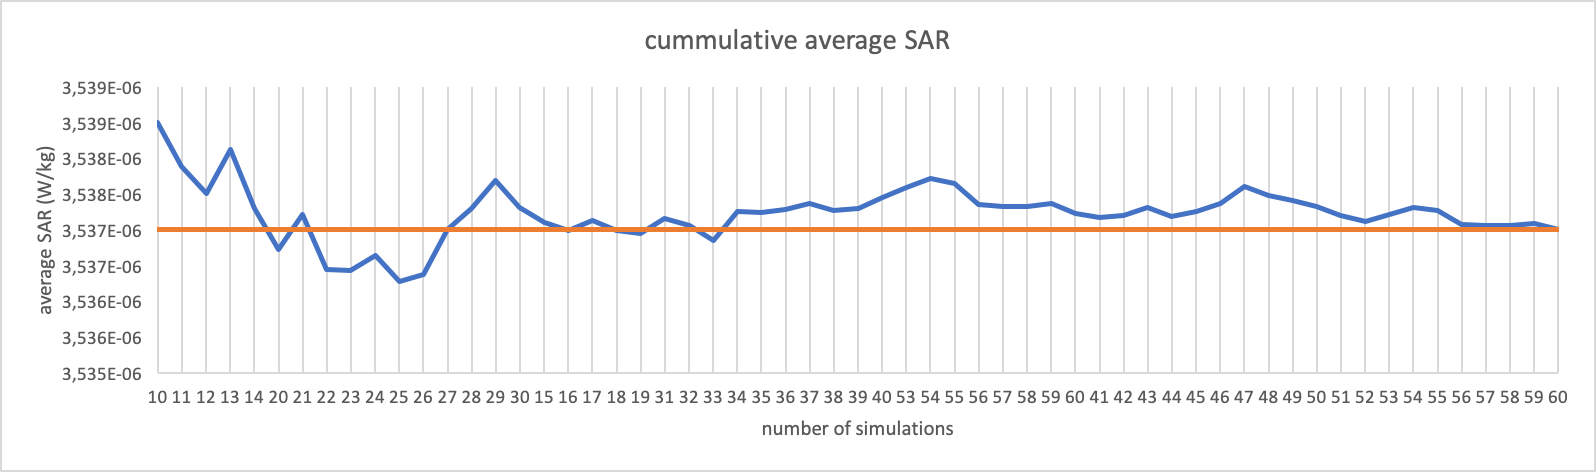
\includegraphics[width=\textwidth]{../results/numberOfSim/sarvssim.png}
  \caption{Total SAR versus.}
  \label{fig:fhsar}
\end{figure}
\begin{figure}[th!]
  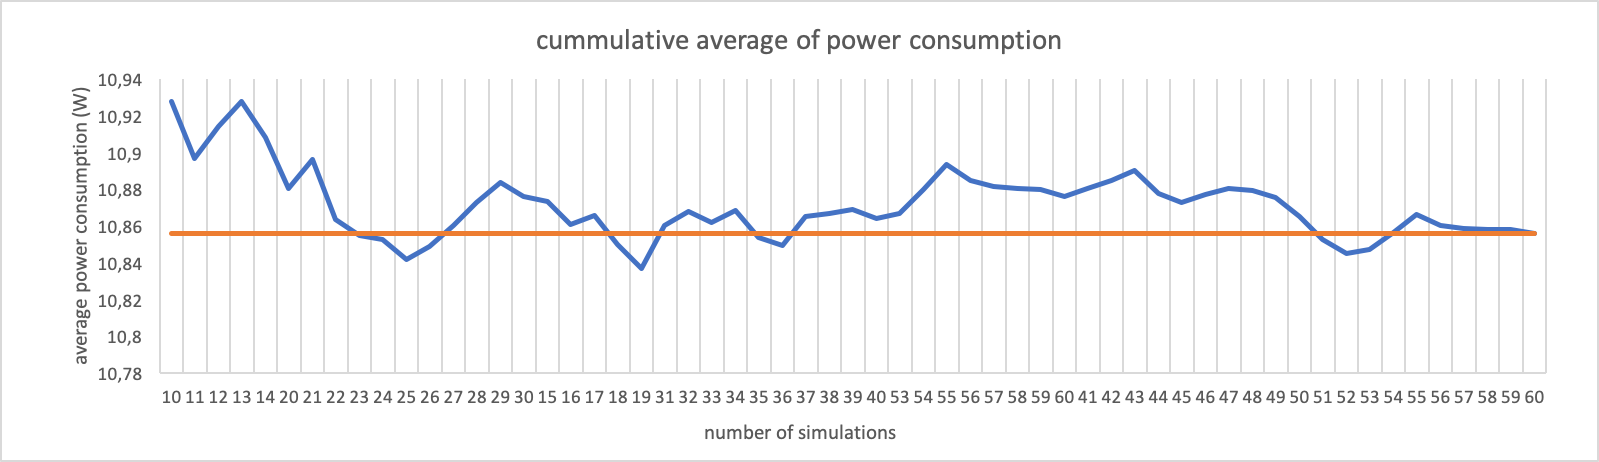
\includegraphics[width=\textwidth]{../results/numberOfSim/pcvssim.png}
  \caption{General design of a microstrip antenna.}
  \label{fig:fhsar}
\end{figure}
\begin{figure}[th!]
  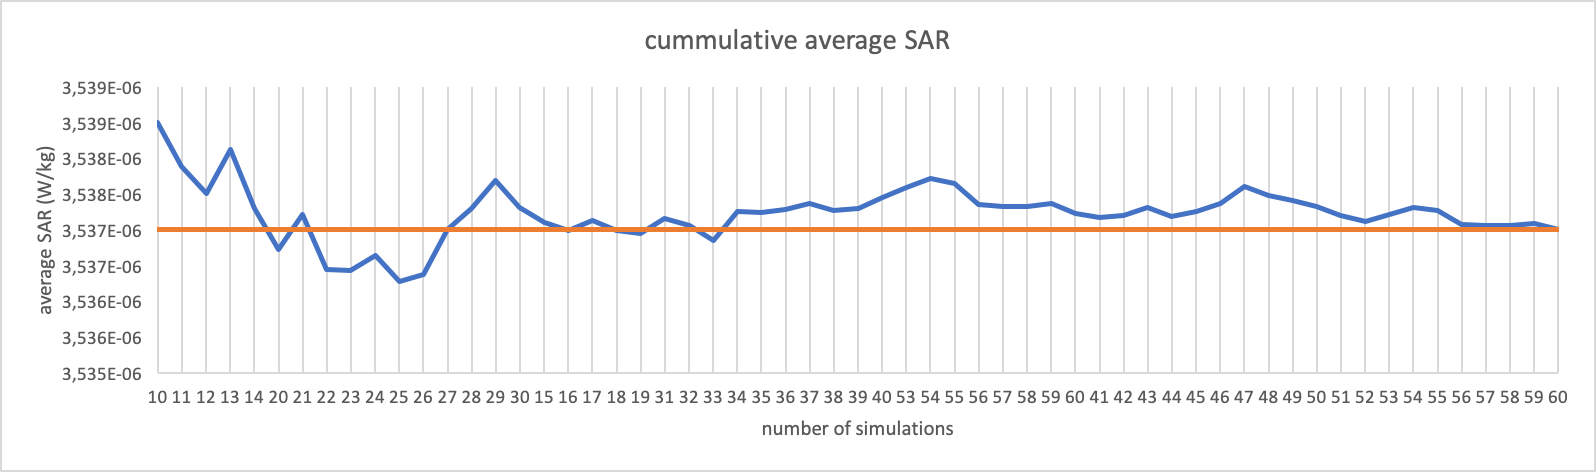
\includegraphics[width=\textwidth]{../results/numberOfSim/sarvssim.png}
  \caption{General design of a microstrip antenna.}
  \label{fig:fhsar}
\end{figure}
\fi %remove to reanable section
%%%%%%%%%%%%%%%%%%%%%%%%%%%%%%%%%%%%%%%%%%%%%%%%%%%%%%%%%%%%%%%%%%%%%%%%%%%%%%%%%%%%%%%%%%%%%%%%%%%%%%%%%%%%%%%%%%%%%%%%%%%%%%%%%%%%
\section{Scenario 1: One User and One Drone}
The network contains only one user for this scenario. This means that there is only one location possible for the drone which is just above 
the user. This section will investigate minimal required transmission power and SAR values from different sources.
\textcolor{red}{power consumption te doen}

\subsection{The Influence of the Maximum Transmission Power}
\label{s1a}
\gls{LTE} makes usages of power control meaning that no more power will be used then strictly necessary. The actual 
transmit power $P_{tx}$ therefore ranges between 0 and the maximum input power. $P_{tx}$ is zero when the \gls{UABS} doesn't cover anybody.
For instance when the flying height is too high and therefore also the path loss that comes with it, the maximum allowed $P_{tx}$ is not enough to cover 
the distance. In such case, the \gls{UABS} is shut down since it cannot meet the requirements.
Increasing the maximum transmission power won't influence the actual used $P_{tx}$ or $SAR_{10g}$ because the \gls{UABS} won't use more
then strictly required. It is therefore more useful to match the actual transmission power against a variable flying height. 

Figure \ref{fig:ptxfh} shows the logarithmic relationship between $P_{tx}$ and flying height.
As already discussed in \ref{sec:s1}, the user is outdoor and just below the \gls{UABS}. There is thus a free line-of-sight between both
radiators. It is clear  from figure \ref{fig:ptxfh} that a discontinue step function is achieved. This is because multiple flying heights correspond to the same transmission power.
When the flying height increases, so does the path loss. \gls{LTE} tries to counteract this by increasing the power level. Each time 
the path loss becomes too high, the power level of the antenna increases with one dBm. Doing so, decreases path loss allowing the antenna to reach
the user again. 

\begin{figure}[t]
  \centering
  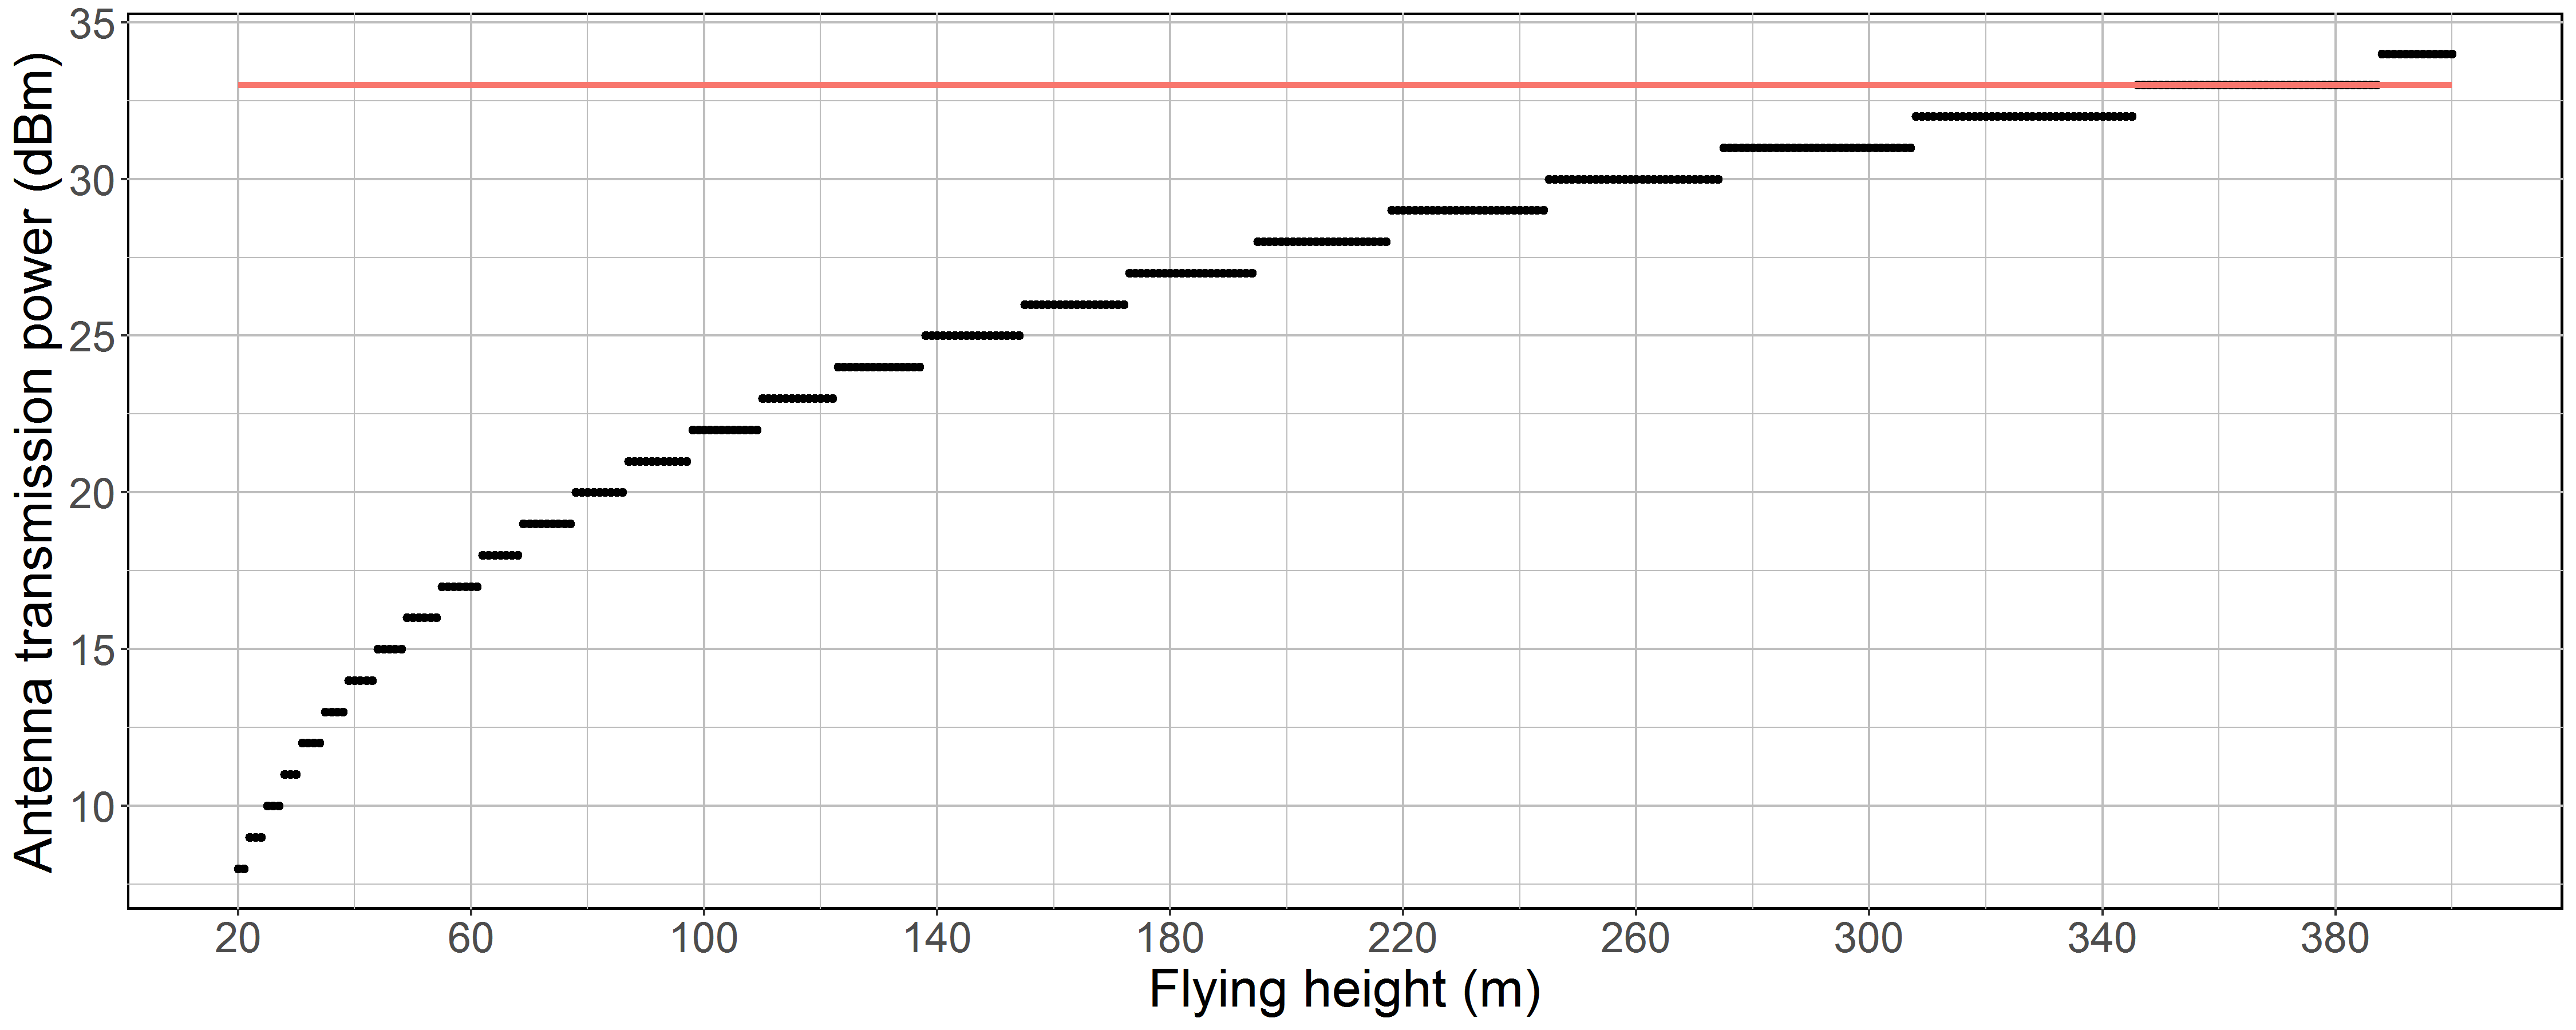
\includegraphics[width=\textwidth]{../results/s1/ptx.png}
  \caption{Minimal required transmission power by the antenna to reach the ground just below him. The red line shows the default maximum transmission power.}
  \label{fig:ptxfh}
\end{figure}

After a jump in the step function, there is an overestimation meaning the input power increased more then necessary. So multiple flying heights correspond with the same $P_{tx}$.
Further, dBm is also a logarithmic scale meaning that while 10 dBm equals 10 mW, 20 dBm equals 100 mW. This explains why the black lines become longer at higher flying altitudes.
Each time the power level increases with one dBm, the overestimation becomes larger. If the tool would make usage of a smaller step size, a more continuous 
logarithmic function would be achieve. This would however worsen the time complexity because it would take much more iterations before 
the power level exceeds the path loss. 

The red line in figure \ref{fig:ptxfh} indicates the default maximum transmission power used during simulations. 
In a free line-of-sight scenario with only one user, a \gls{UABS} can fly up to 387 meters before losing connection.

This scenario is investigated with a microstrip patch antenna using power consumption optimization. The configuration however does not matter
despite the fact that an \gls{isotropicradiator} doesn't have any attenuation while a microstrip patch antenna does.
Since the user is positioned in the perfect center of the main beam where there is 
no attenuation experienced in either cases. Also the optimization won't make a difference. The goal of the optimization strategy is to decide which 
drone is most suitable for which users. Since there is only one user and one possible position for the drone, both optimization strategies behave identical.

\FloatBarrier
\subsection{Influence of the Flying Height}
\label{sub:senario1_influenceOfFlyHeight}

This section investigates how the flying height of a \gls{UABS} influence $SAR_{10g}$ and power consumption.
This induced electromagnetic radiation for our user is represented in figure \ref{fig:s1_fhsar}
and shows that for low flying drones, \gls{UABS}s are the main source of electromagnetic radiation (green line).
This changes around 80 meters where the \gls{UL} electromagnetic radiation of the \gls{UE} (red line)
exceeds the \gls{DL} radiation in order to still be able to reach the high flying \gls{UABS}s.

\gls{SAR}-values are caused by the input power of the antenna. The $P_{tx}$ in section \ref{s1a}
showed a discontinue behaviour that sometimes radiate more as strictly necessary. This has thus a direct influence
on  $SAR^{dl}_{10g}$. Hence the same discontinue behaviour. $SAR^{dl}_{10g}$ can be simplified to an perfect constant line.
This constant behaviour can once again be explained with power control. When the \gls{UABS} flies lower, there is  less path loss. The \gls{UABS} 
will therefore reduce $P_{tx}$. This results in formula \ref{eq:exposureBasicFormula} where the electromagnetic exposure is a constant fraction of power and distance.

\begin{equation}
\vec{E} (V/m) = \frac{\Delta U (V) }{\Delta x (m)}
\label{eq:exposureBasicFormula}
\end{equation}

The SAR values are the result of multiplying the electromagnetic exposure with a constant as explained in equation \ref{eq:DLconvertion}.
So both have a linear relationship.

Figure \ref{fig:s1_fhsar} doesn't show radiation from neighbours, because there are none present in this scenario. 
Finally, all these values are added as explained in formula \ref{eq:overallSARwb} and indicated with the blue line. 

\begin{figure}[]
  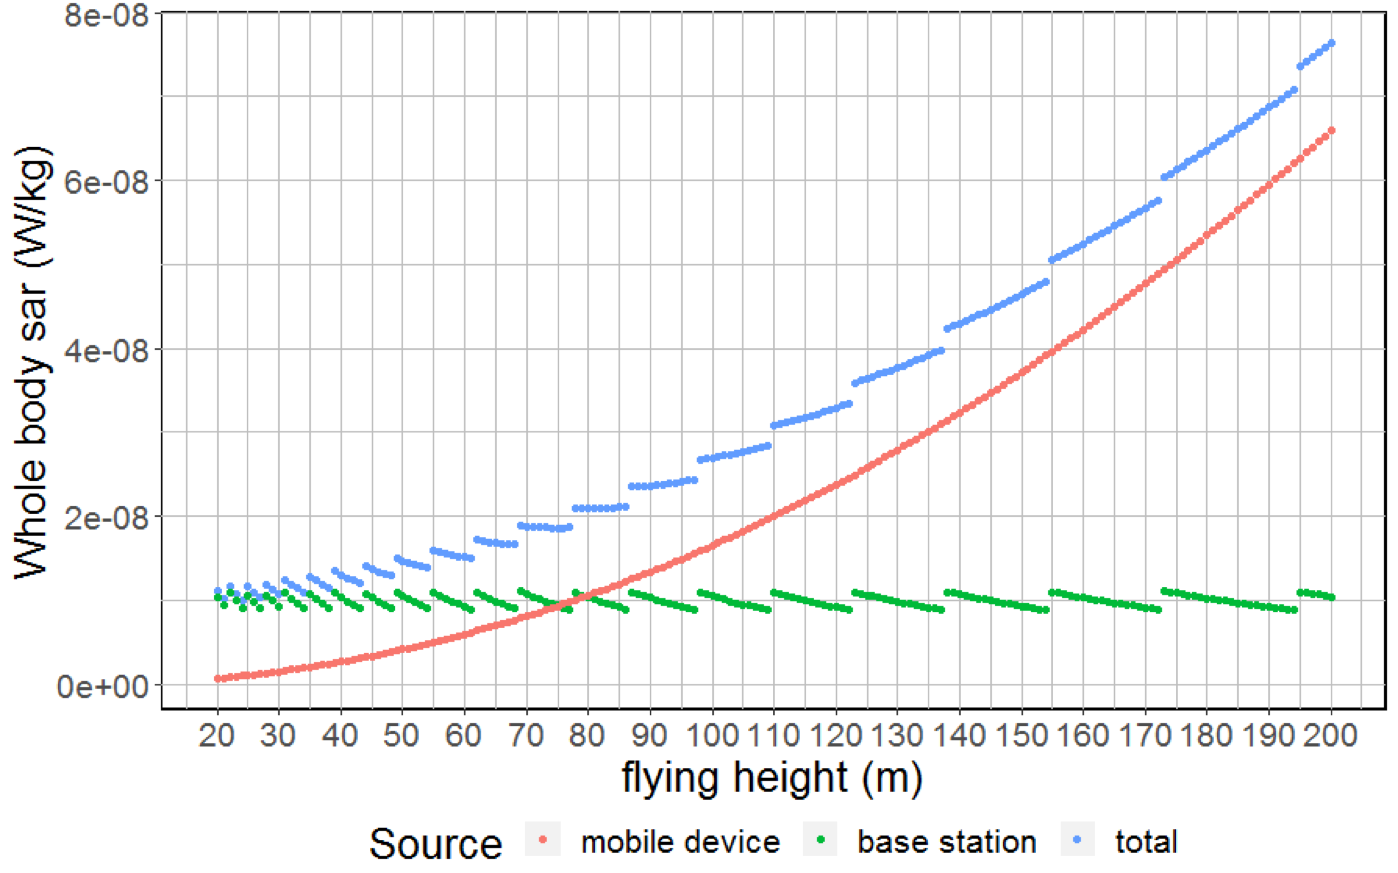
\includegraphics[width=\textwidth]{../results/s1/fhvssar2.png}
  \caption{How SAR values from different sources are influenced by different flying altitudes.}
  \label{fig:s1_fhsar}
\end{figure}

\textcolor{red}{power consumption te doen}
%%%%%%%%%%%%%%%%%%%%%%%%%%%%%%%%%%%%%%%%%%%%%%%%%%%%%%%%%%%%%%%%%%%%%%%%%%%%%%%%%%%%%%%%%%%%%%%%%%%%%%%%%%%%%
\FloatBarrier
\section{Scenario 2: Increased Traffic}

This scenario has just like the previous scenario only one drone available. However, more users will be present in the network.
First, a variable flying altitude is investigated for a fixed number of 224 users. 
Secondly, the flying height is set to 100 metres with a variable number of users.
When designing the network, there will be as much possible drone locations as there are users in the network and the tool
will consider all of them. It's only when the programme is finished, that one drone remains.

\subsection{Influence of the Flying Altitude}
This scenario investigates how the network consisting out of one \gls{UABS} behaves when applied on an ordinary day during rush hour. 
On average, 224 active users are distributed uniformly over the city center of Ghent. 
Figure \ref{fig:s2a_dlAndPc} shows how the downlink exposure is clearly influenced by the flying height of the \gls{UABS}. 
This is because if a drone flies higher, there is less penetration loss from obstructing buildings.

A power consumption optimized network with an \gls{EIRP} antenna (green) has the highest exposure. 
This is logical when comparing with an EIRP antenna in an exposure optimized network (red). 
However, when looking at figure \ref{fig:s2a_dlAndPc} on the right, the power consumption in a power consumption optimized network is worse 
than in an exposure optimized network. To understand this, the behaviour of the deployment tool needs to be understood first. 
A power consumption optimized network will result in a few high powered \gls{UABS}s because increasing the input power of an antenna cost 
less then activating a new  drone. Likewise, an exposure optimized network 
generates a lot of low powered \gls{UABS}s because the lower the antenna's power, the lower the exposure. This has the consequence that the cover radius 
is less and therefore requiring more drones which costs more energy.
When only a limited amount of \gls{UABS}s are available, 
like only one in this scenario, the tool will only keep \gls{UABS}s which cover most of the users. 
Therefore is the power consumption in a power consumption optimized network way higher. 


\begin{figure}[h!]
  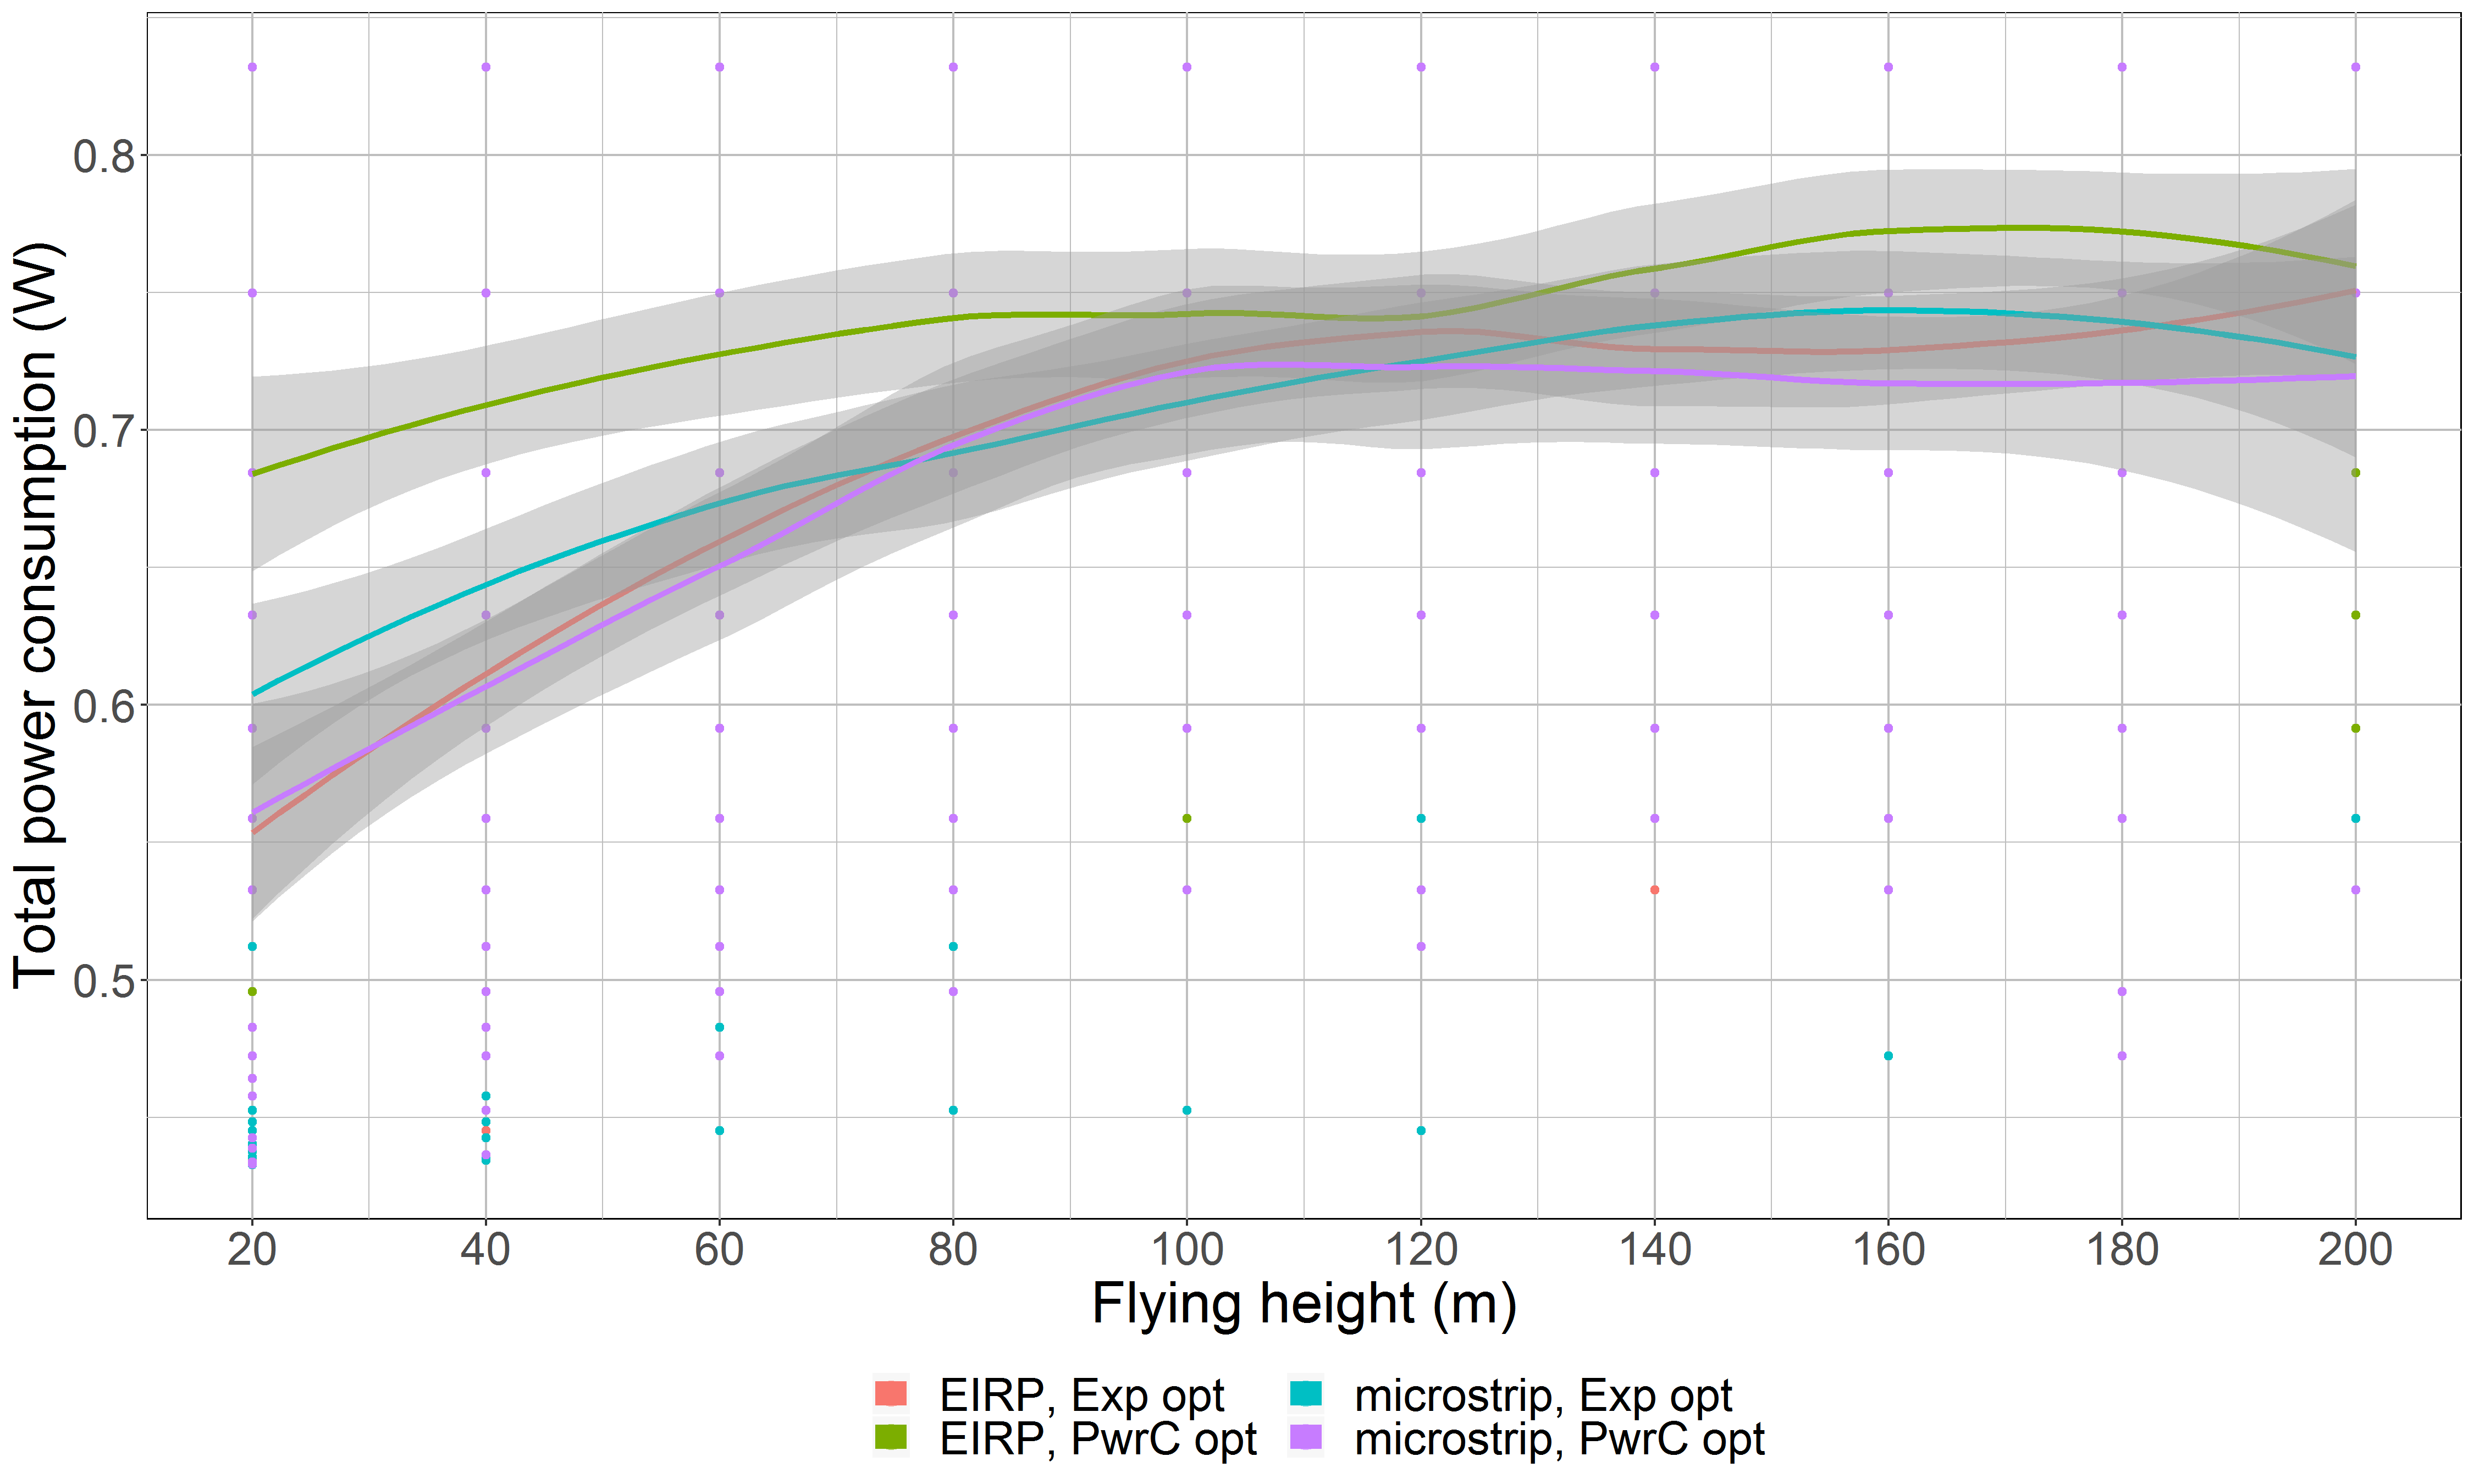
\includegraphics[width=\textwidth]{../results/s2/fhvsdlAndPc.png}
  \caption{The influence of the flying height on the weighted average downlink exposure of users in the network.}
  \label{fig:s2a_dlAndPc}
\end{figure}

\begin{figure}[bh!]
  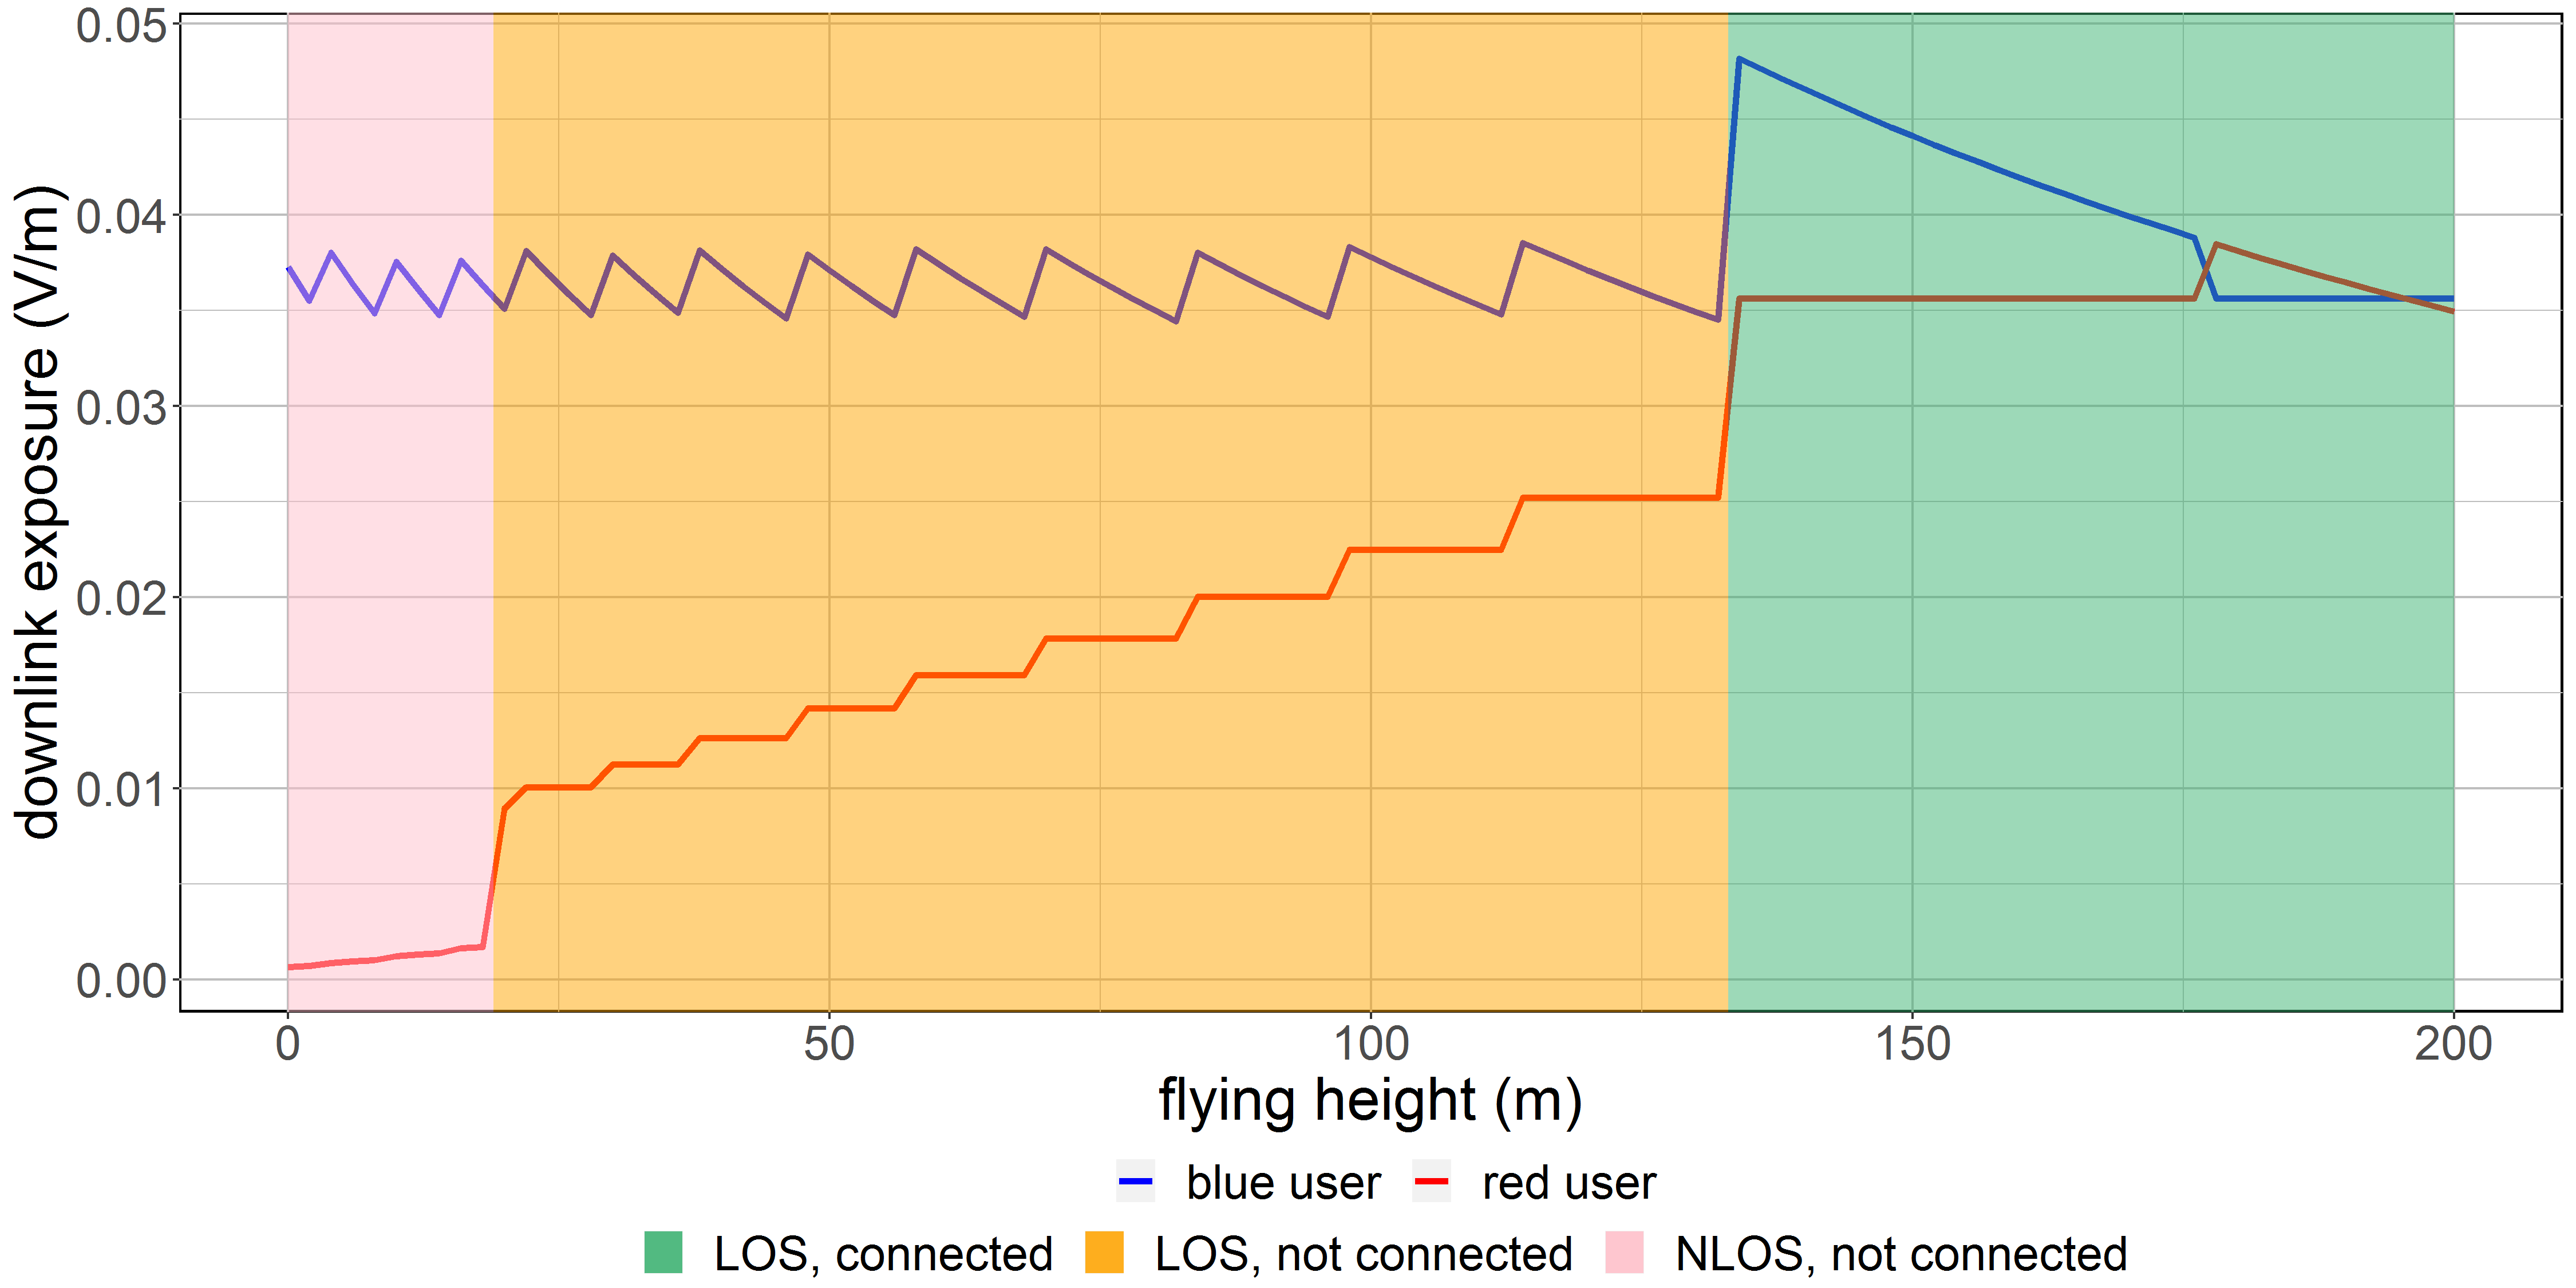
\includegraphics[width=\textwidth]{../results/s2/prove.png}
  \caption{Scenario 2 with only 2 users. The coloured areas are only applicable for the orange user. The blue user is connected during the entire time.}
  \label{fig:prove}
\end{figure}


\begin{wrapfigure}{r}{0.49\textwidth}
  \begin{center}
    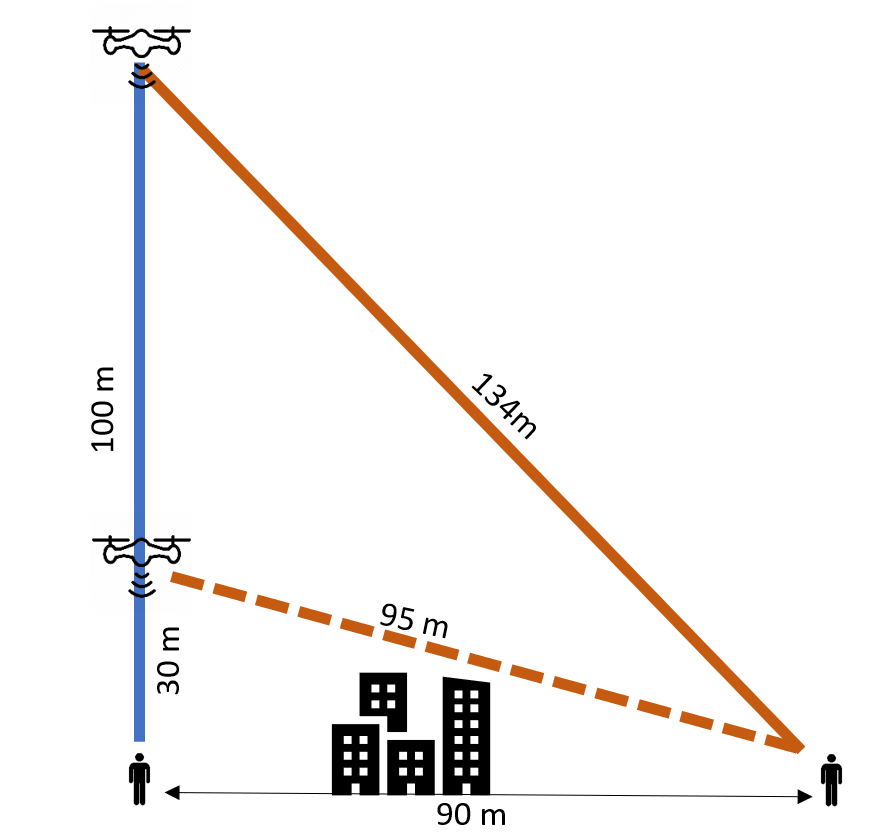
\includegraphics[width=0.48\textwidth]{../results/s2/proveScenario.png}
  \end{center}
  \caption{Schematic overview of scenario 2 with only 2 users.}
  \label{fig:schematicprove}
\end{wrapfigure}

\newpage
The correctness of the exposure in figure \ref{fig:s2fhvsdl} is proven with figure \ref{fig:prove} by investigating the scenario with only two users. The two users who 
will be referred to by `red' and `blue' are 90 metres separated from each other with a building between them.
Scenario 1 already explained that the charts can be simplified and the blue line from fig. \ref{fig:prove} remains in fact constant between the zero and 130 metres.
The chart shows that the \gls{UABS} is positioned above the blue user. The orange user is in \gls{NLOS} as long as the \gls{UABS} remains below 20 metres.

Once the \gls{UABS} increases its flying altitude, the orange user becomes into \gls{LOS} but still remains uncovered. This is because the tool initially locate a possible 
\gls{UABS} above each user and thereafter performs the  fitness function. The applied fitness function must have decided that it is better to connect 
each user to the \gls{UABS} above him. At a final state, the tool check whether the number of online drones does not exceed the capacity of the facility
which is here the case. The tool therefore deactivates one \gls{UABS} causing the orange user to be uncovered. One could argue that the 
the orange user should be connected to the online drone who is only 90 metres away. This would however require the online drone to increase his power consumption which 
would make the decisions made by the optimization strategy obsolete.
When the drone flies higher, the difference in distance between both users and the base station decreases. In other words, the Pythagorean theorem shows that when the flying height of the 
\gls{UABS} increases, the distance with the blue user increases faster compared to the distance between that same \gls{UABS} and the orange user. This is also illustrated in figure \ref{fig:schematicprove}.
At 130 metres, the tool decides to connect both users to the same \gls{UABS}. Therefore, it increases it's power consumption so the orange user would  have the minimal 
required electromagnetic exposure.This has of course a negative influence for the blue user who is way closer and experience now a much higher exposure level  (fig. \ref{fig:prove}).
Around 180 metres, the  orange and blue line switch because the drone changes position. As explained before, the tool assigns two possible drones, one above 
each user. The tool must have decided that connecting both users to the other drones improves the fitness function of the entire network even though that difference might be 
very little.
The electromagnetic exposure in figure \ref{fig:fhvsdlAndPc} is the weighed average of all users. In other words, there are 223 users who behave like the  orange user while only
one user behaves like the blue one. The similarity between the orange line from fig. \ref{fig:prove}  and  the electromagnetic exposure in fig  \ref{fig:s2a_dlAndPc} is clear.

Figure  \ref{fig:s2fhvscov} shows that the flying height has a positive influence on the user coverage. 
When a \gls{UABS} flies higher, there is less path loss between the user and the drone caused by buildings but also the path loss to neighbouring 
users decreases as explained 
with figure \ref{fig:prove} and \ref{fig:schematicprove}. 
Also the increasing \gls{DL} exposure  from figure \ref{fig:s2a_dlAndPc} confirms the that the
user coverage should grow.
As mentioned before, a power consumption optimized network will result in few high powered \gls{UABS}s. 
The tool removes all \gls{UABS}s except the one with most users. 
The network therefore exist out of one high powered \gls{UABS} compared to the exposure optimized network with one drone which 
will be less powered. Since green has a higher power level, also more users will be covered.

When replacing the fictional \gls{EIRP} antenna with a microstrip patch antenna, the percentage of covered users drops for both 
optimization strategies. This is because users who have a higher horizontal distance between themselves and the \gls{UABS}, 
experience a higher attenuation. Also, when a microstrip patch antenna is positioned higher, the range of the antenna increases 
since the angle between the user and the \gls{UABS}s main lob decreases. The user will therefore experience less attenuation.

%It becomes also clear that this advantage is limited. For a scenario of 224 users and one drone, the user coverage won’t increase
% significantly any more around an altitude of 120m.

\begin{figure}[h!]
  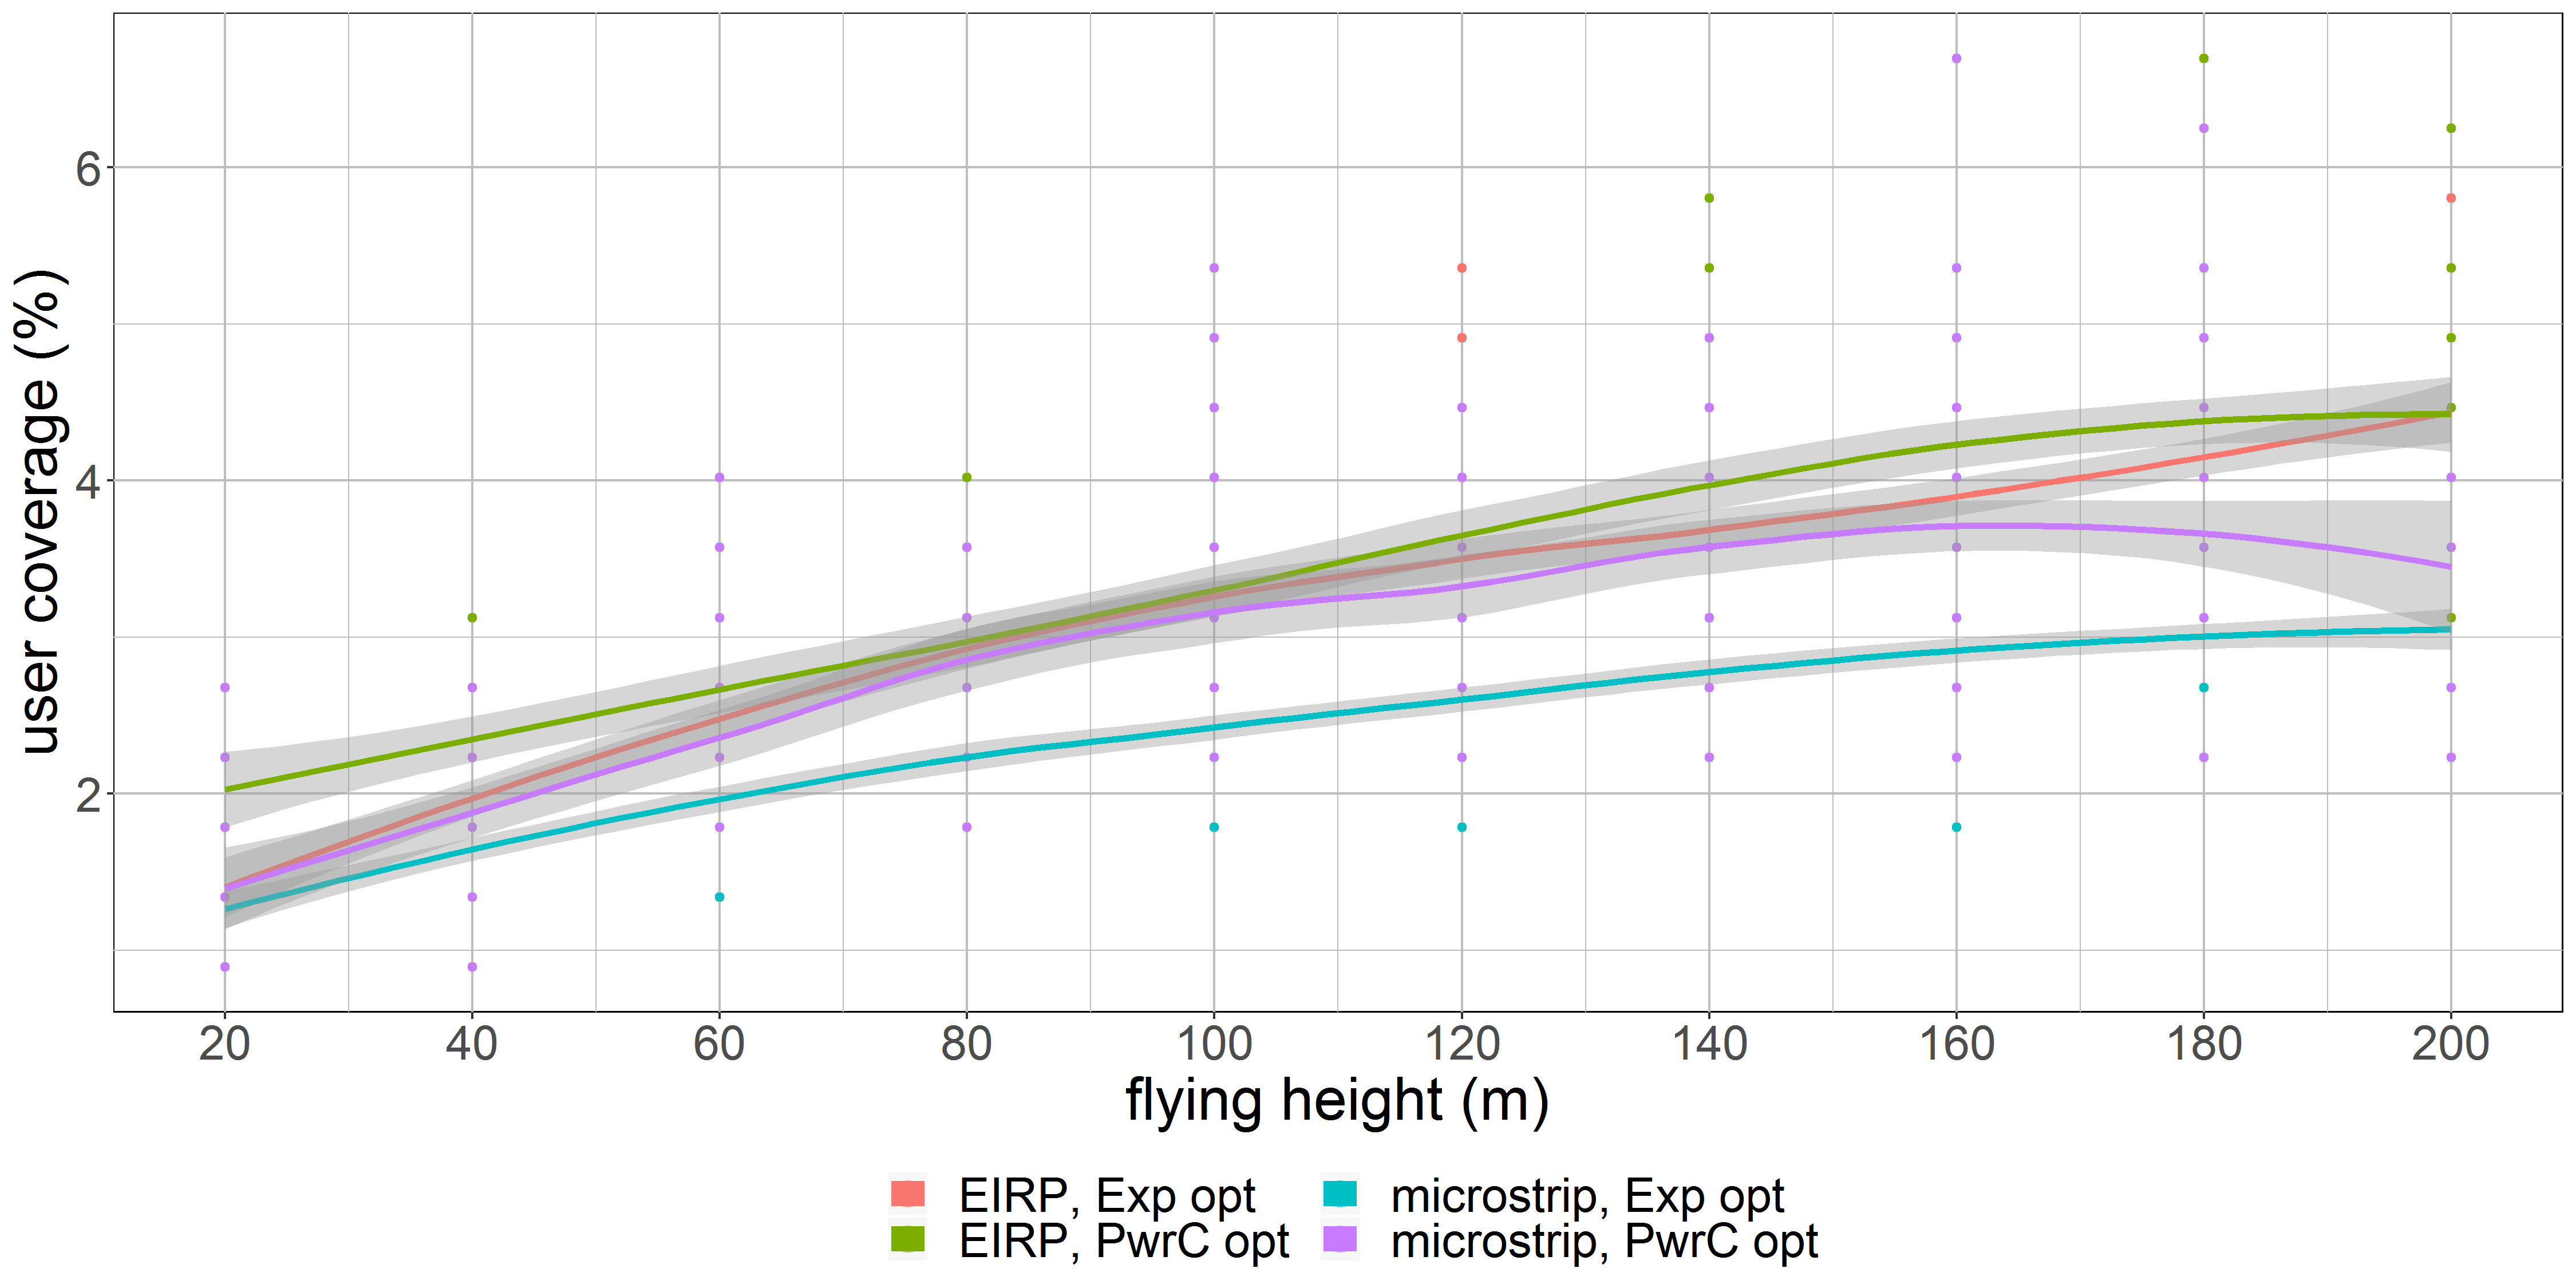
\includegraphics[width=\textwidth]{../results/s2/fhvscov.png}
  \caption{This graph shows the percentage of covered users by one drone for different flying heights.}
  \label{fig:s2fhvscov}
\end{figure}

Figure \ref{fig:s2fhvssar} shows the total whole body SAR10g, deducted from all electromagnetic sources. This being exposure of all \gls{UABS}s,
 the uplink exposure from the user’s own device and the exposure of the devices from all other users. 
 Thereafter, the weighted average of all whole body SAR10g values in the network is calculated with the 50th and 95th percentile 
 being the most important values. This is because not only the mean values are important but also users who experience higher 
 levels of whole body SAR10g.


\begin{figure}[h!]
  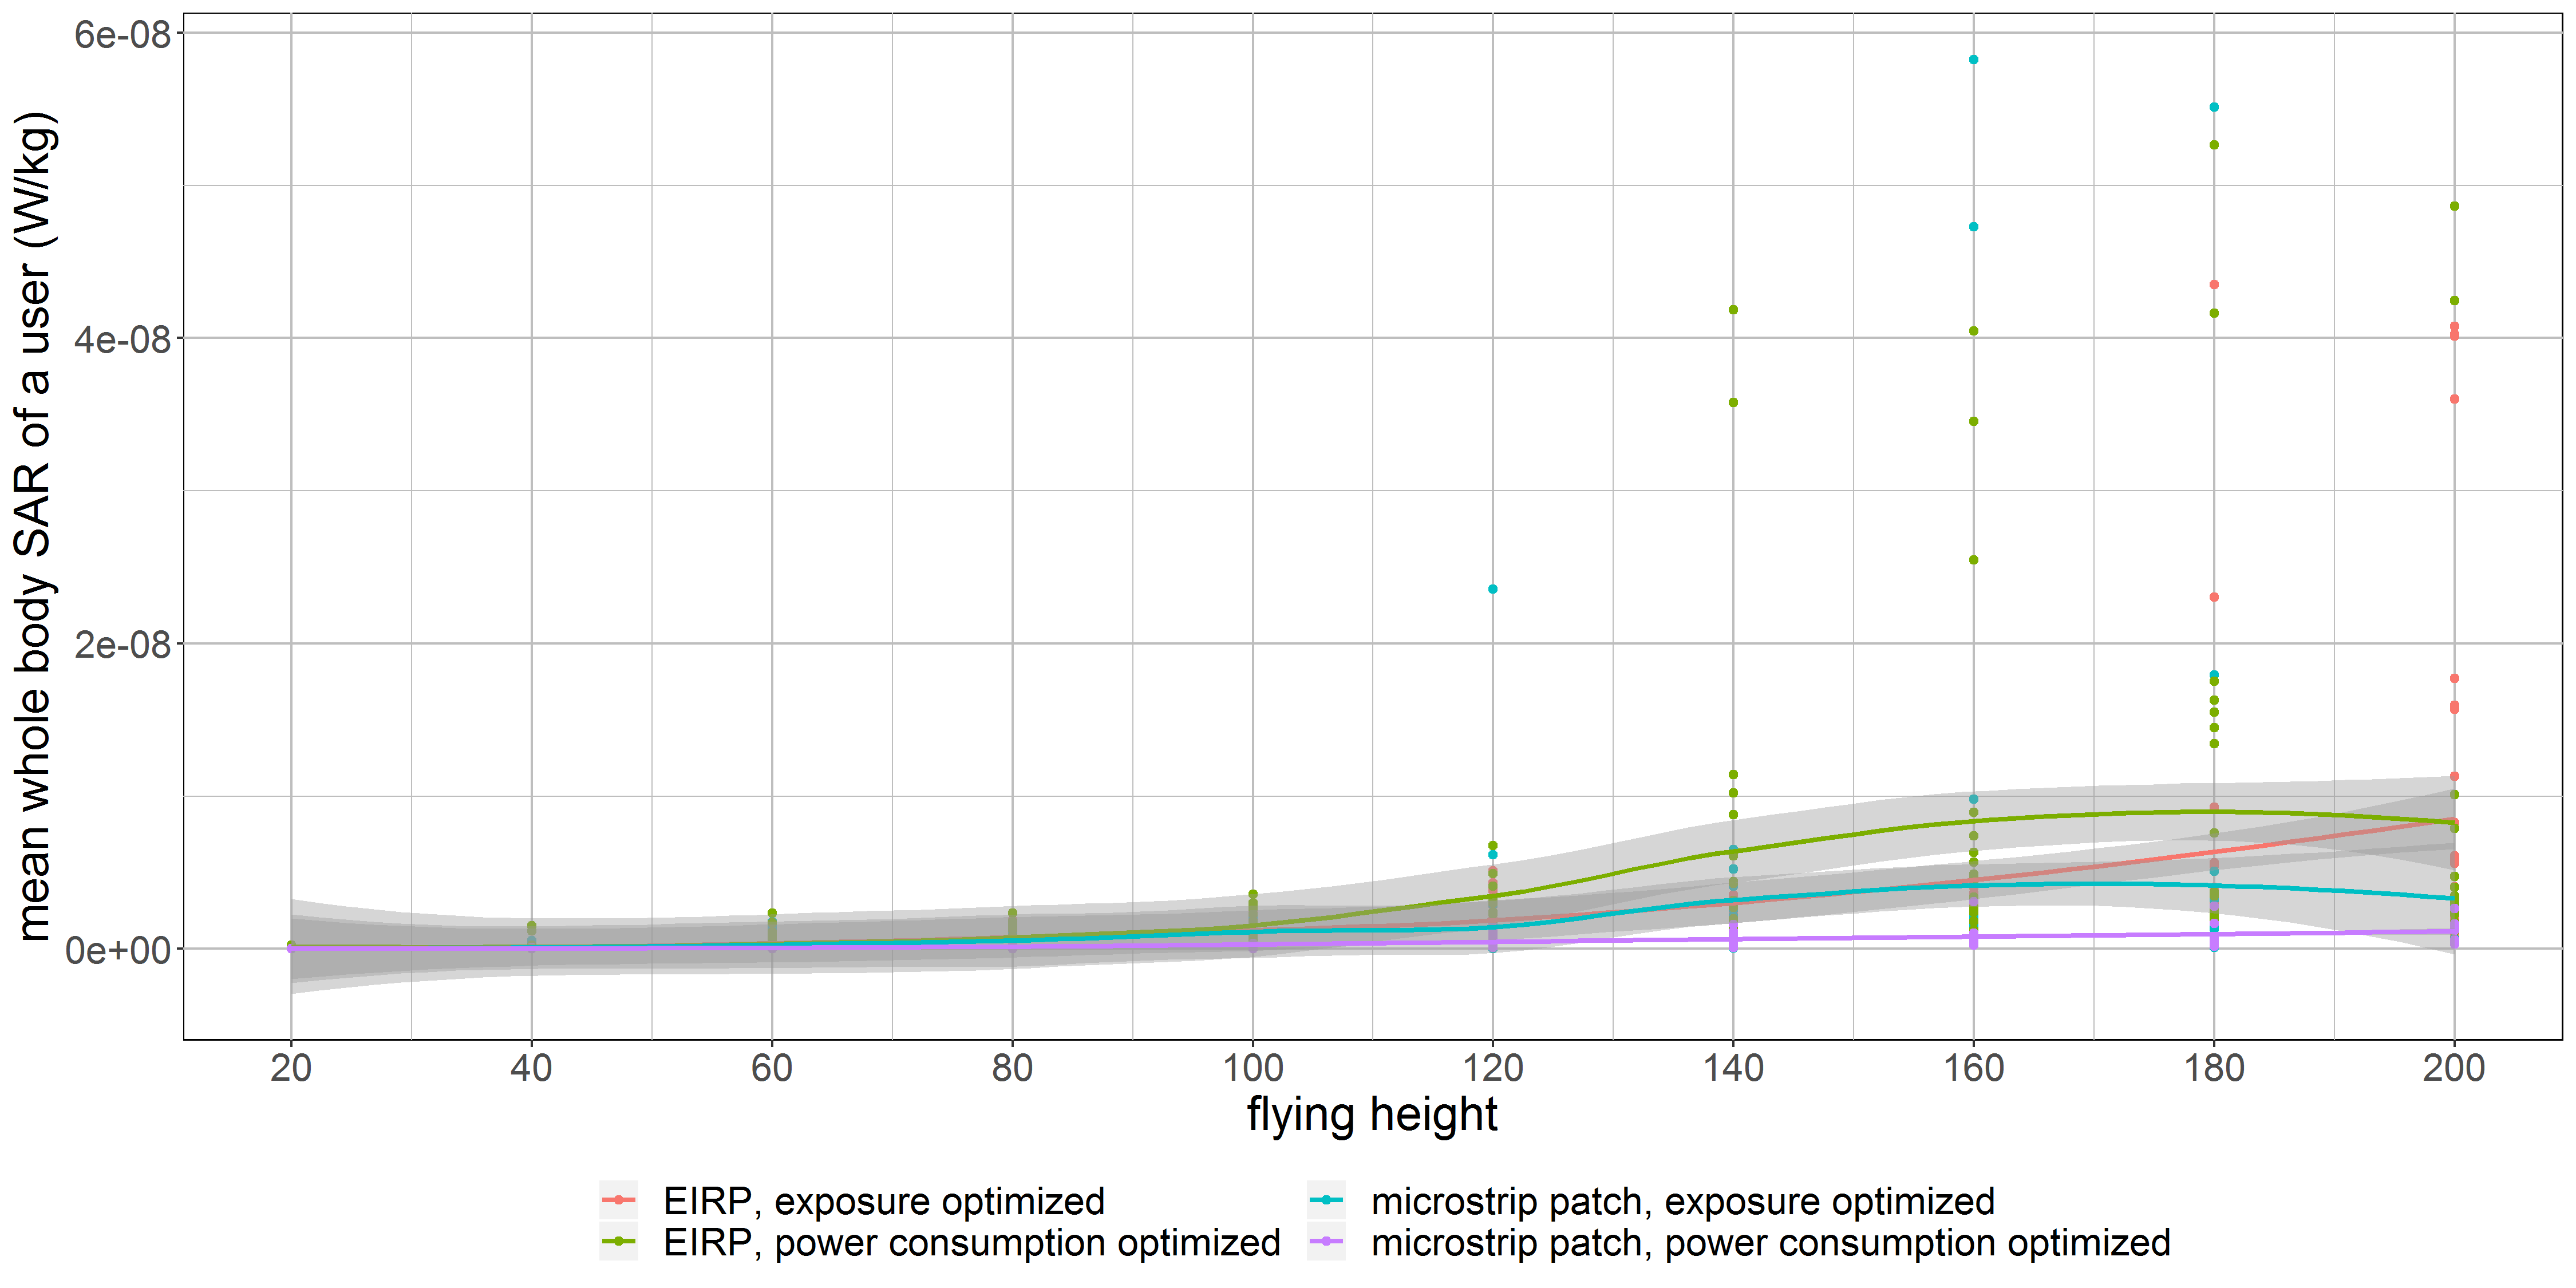
\includegraphics[width=\textwidth]{../results/s2/fhvssar.png}
  \caption{The influence of the flying height on the weighted average $SAR_{10g}$ of users in the network.}
  \label{fig:s2fhvssar}
\end{figure}

When investigating the 3 different sources of which the total \gls{SAR}-values are based on, we see 
that the radiation from the \gls{UABS} is the main factor followed by the near field radiation from the user's own device.
The far field radiation from other \gls{UE} has barely influence. 
It looks like it is zero but it is just very low compared to the other two values and in fact does increases when the flying height becomes larger (just like the two other lines).

The weighted average $SAR^{ul}_{10g}$ from the own device is zero in an exposure optimized network with a microstrip patch antenna which is even lower that the $SAR^{neighbours}_{10g}$.
This is because the coverage in this scenario is so low that the weighted average only consist of uncovered users and an uncovered user his device has no power consumption.
\begin{figure}[h!]
  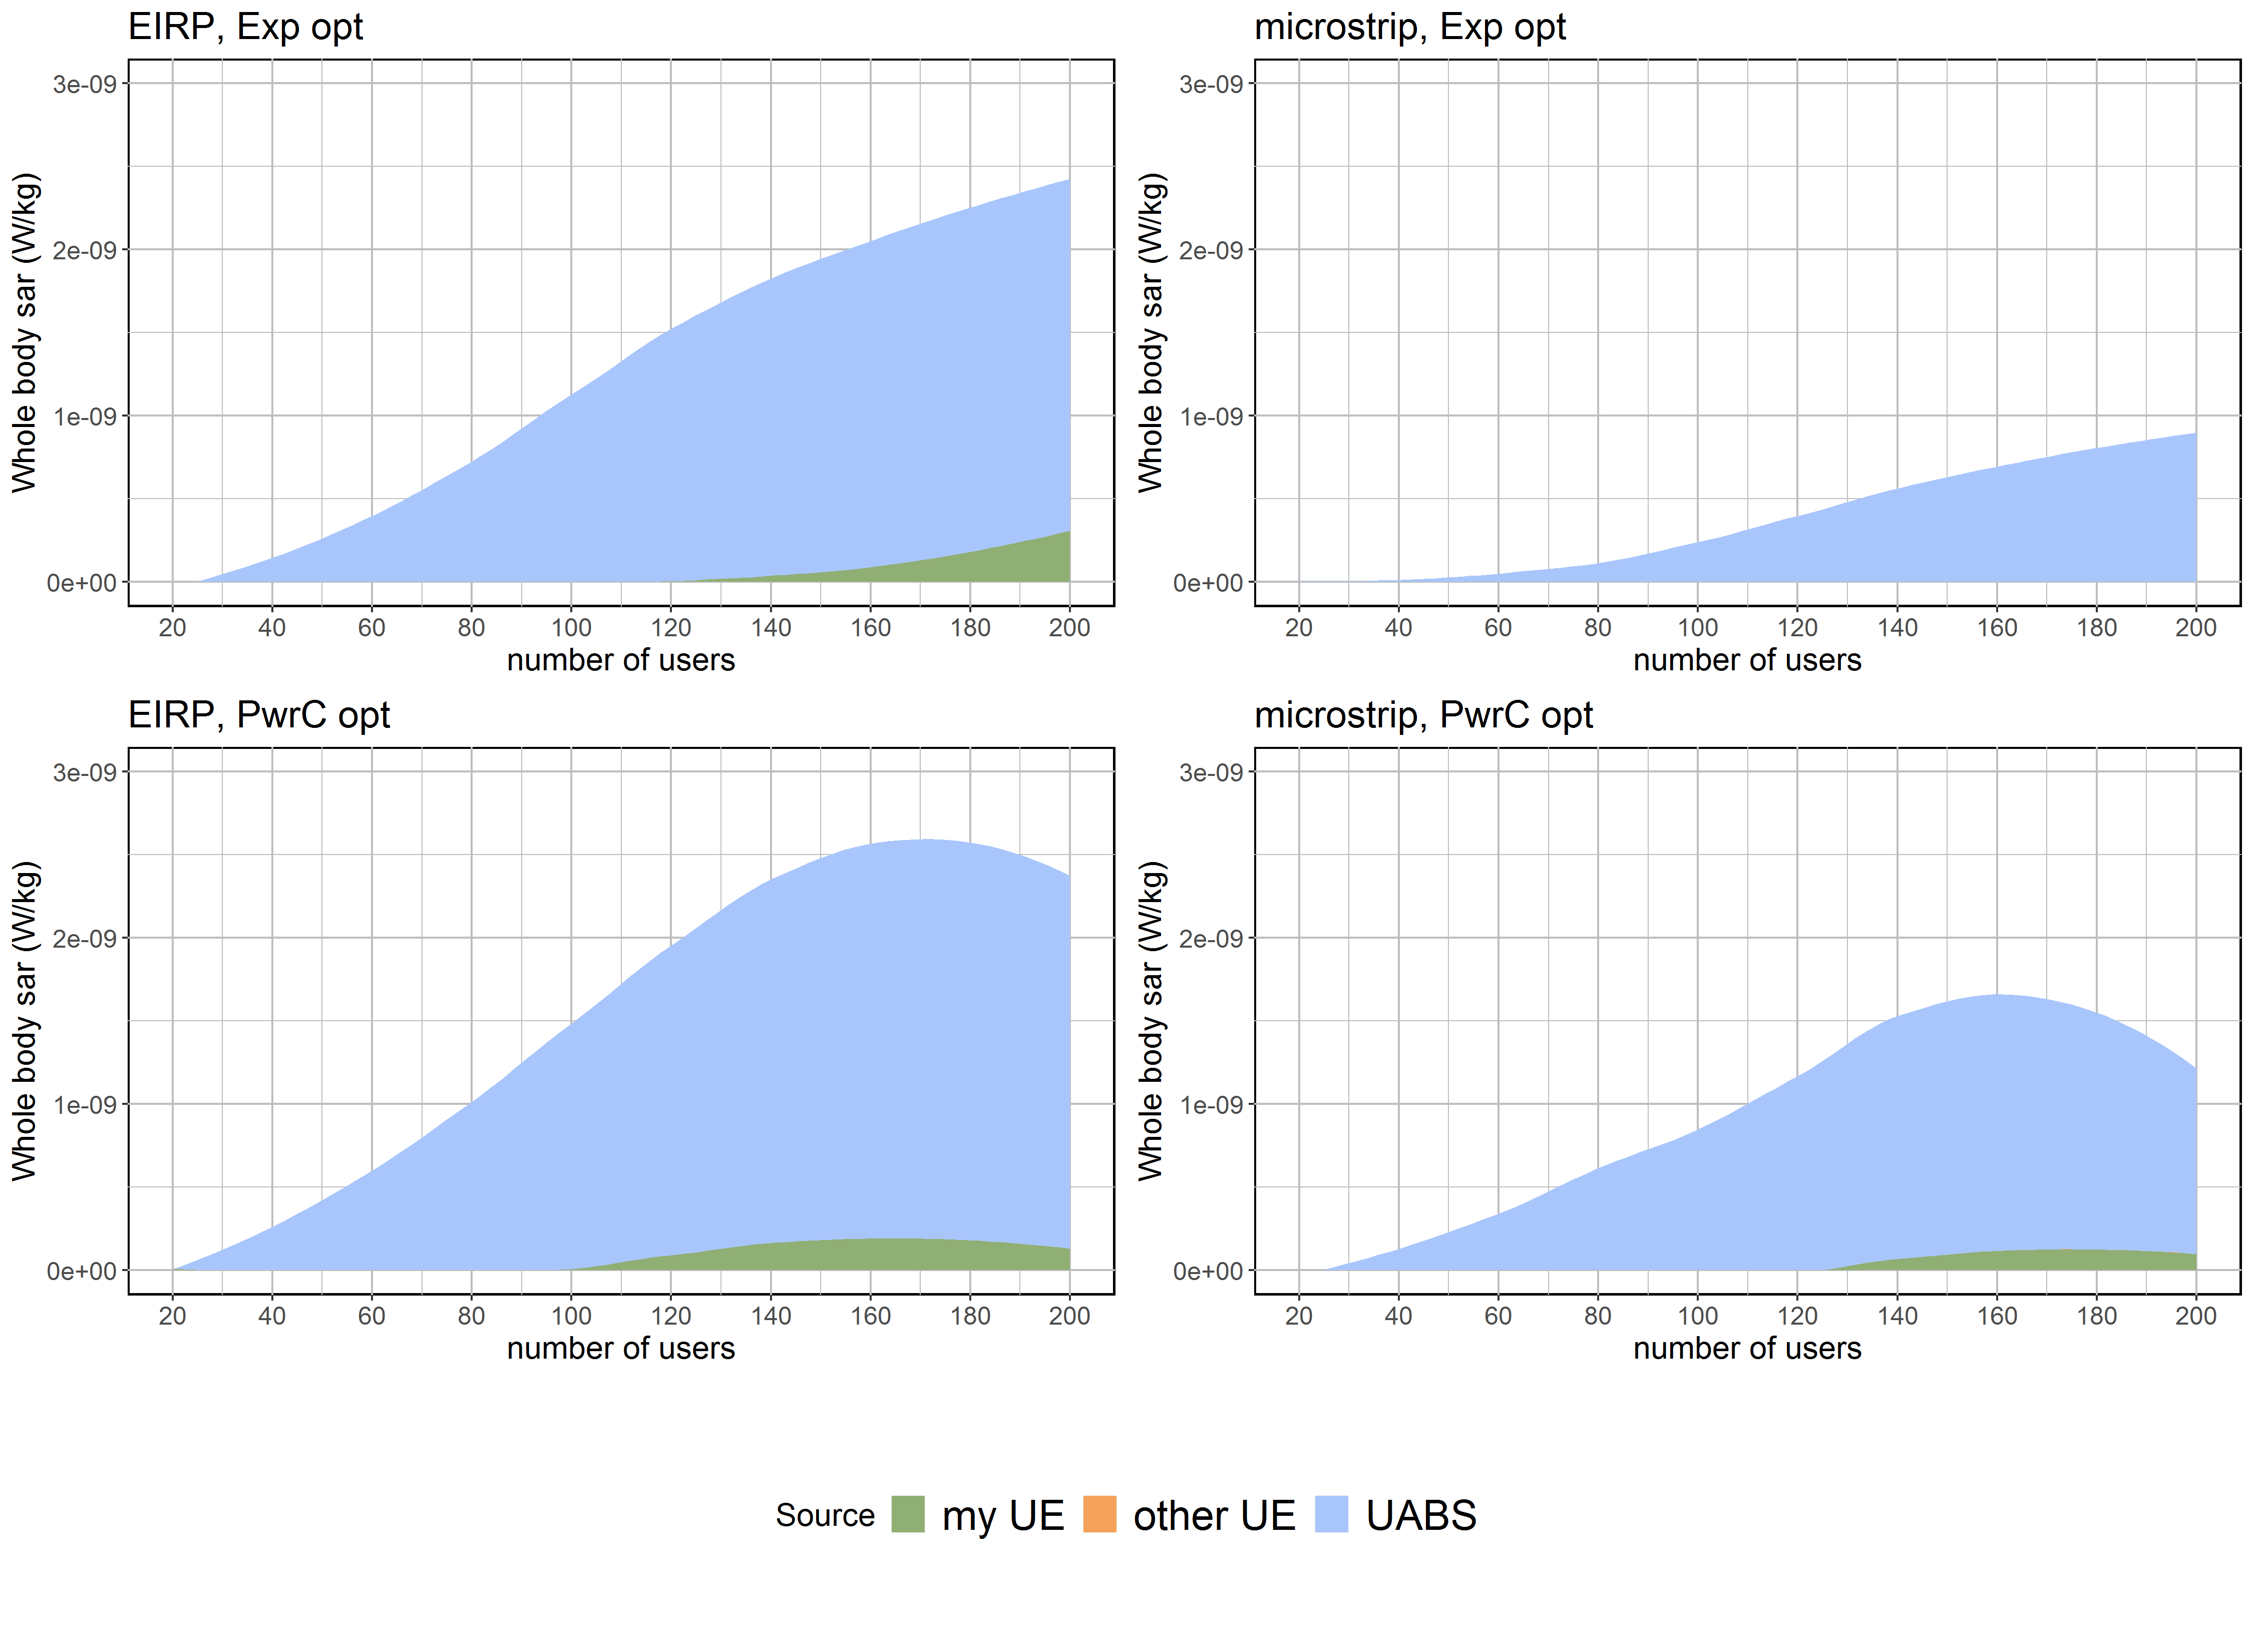
\includegraphics[width=\textwidth]{../results/s2/fhFourSources.png}
  \caption{This figure shows how different sources are influenced by an increasing flying height.}
  \label{fig:s2shfourSourcesMatrix}
\end{figure}

TODO: remove black line


%%%%%%%%%%%%%%%%%%%%%%%%%%%%%%%%%%%%%%%%%%%%%%%%%%%%%%%%%%%%%%%%%%%%%%%%%%%%%%%%%%%%%%%%%%%%%%%%%%%%%%%%
\FloatBarrier
\subsection{Influence of the Number of Users}
\label{s2b}

The number of covered users increase linearly compared to the number of users present in the network. This becomes clear when looking at figure 
\ref{fig:s2uvsnumcovusers} on the right. It shows how an \gls{isotropicradiator} is able of reaching more users then microstrip patch antennae because of the absence of attenuation.
Also, power consumption optimized networks are able of reaching more users compared to exposure optimized networks.
This is because power consumption optimized network will result in few high powered base station where an 
exposure optimized network result in a lot of low powered base stations. This behaviour will further be explained in Section \ref{s3}

This scenario has however only one 
\gls{UABS} at its disposal and only the \gls{UABS} with the most users will remain. The power consumption optimized network therefore exists out of one high powered \gls{UABS} 
while the other optimization strategy has one low powered \gls{UABS}.

\begin{figure}[h!]
  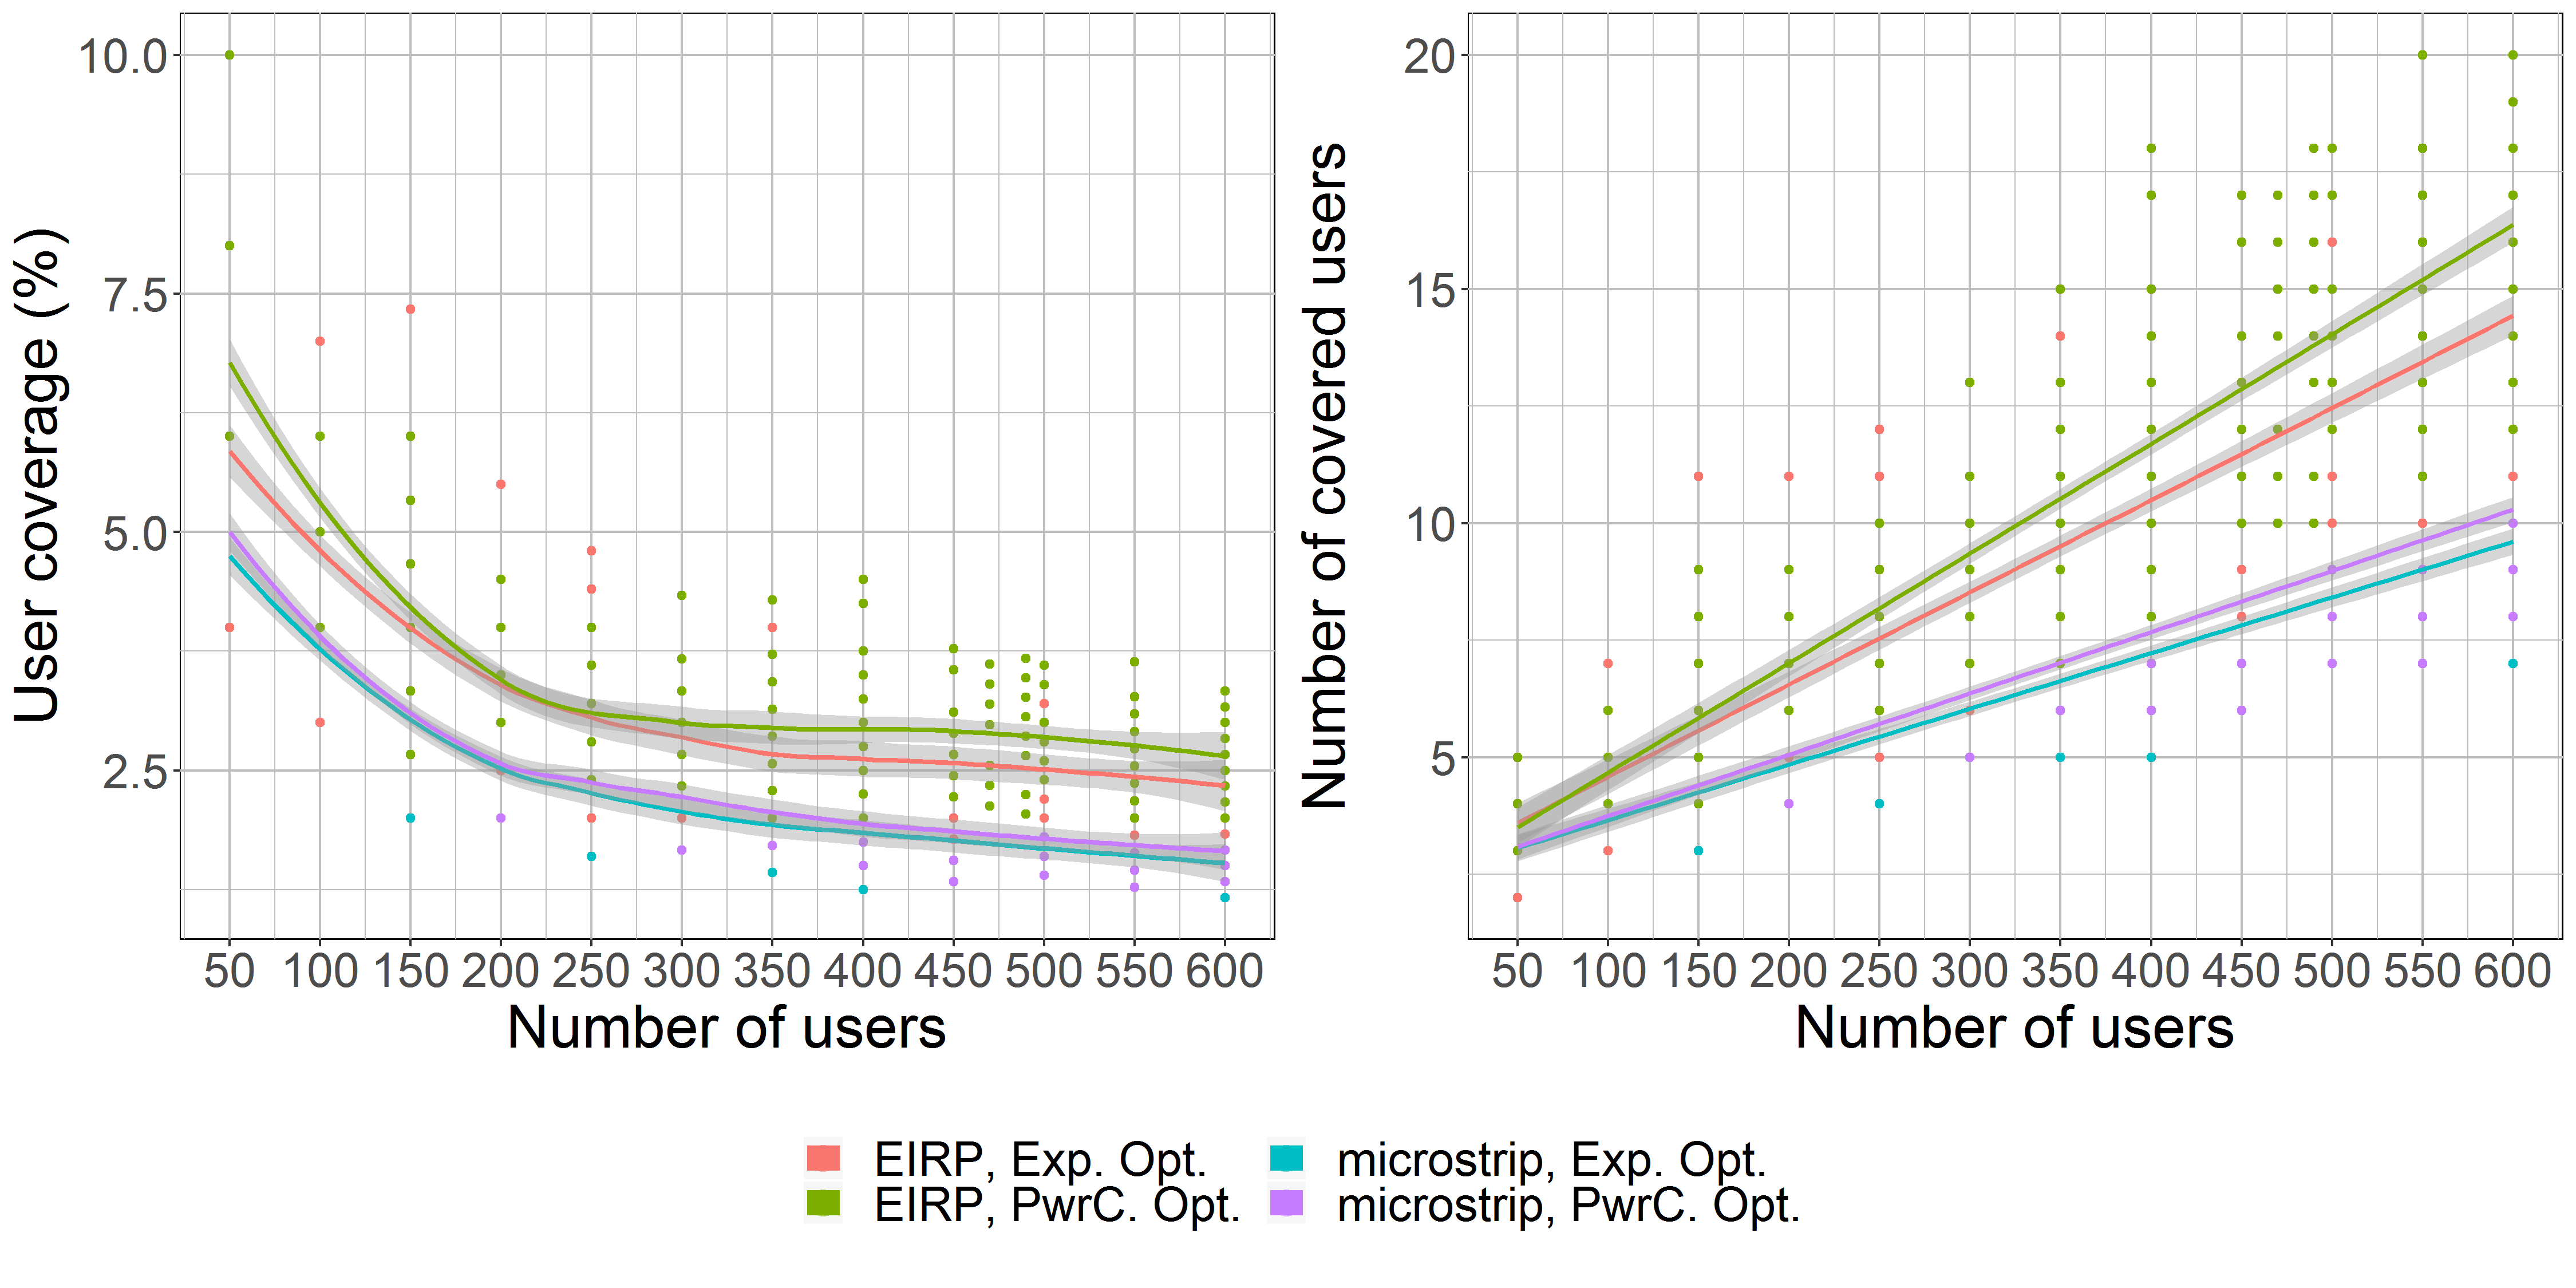
\includegraphics[width=\textwidth]{../results/s2/uvsnumdronesAndCov.png}
  \caption{The influence of increasing traffic on user coverage.}
  \label{fig:s2uvsnumcovusers}
\end{figure}

The linear regression lines from \ref{fig:s2uvsnumcovusers} can be predicted with the equations in \ref{eq:numcovusers}.

\begin{equation}
\text{number of users =}
    \begin{cases}
      y = 0,0233x + 2,3553 & \text{if EIRP and pc}\\
      y = 0,0197x + 2,6144  & \text{if EIRP and exp}\\
      y = 0,0131x + 2,4371  & \text{if micro and pc}\\
      y = 0,0119x + 2,4652  & \text{if micro and exp}
    \end{cases} 
    \label{eq:numcovusers}      
\end{equation}

Figure \ref{fig:s2uvsnumcovusers} on the left show the percentage of covered users that follows out of \ref{fig:s2uvsnumcovusers} on the right by taking the equations from \ref{eq:numcovusers} and dividing them by $x$.
This results in a decreasing logarithmic behaviour because the regression lines from  \ref{fig:s2uvsnumcovusers} have a slope of less then 0.5.
So in other words, the  percentage of covered users for a sparsely populated network is more compared to the percentage of users in high dense populations.

\begin{figure}[h!]
  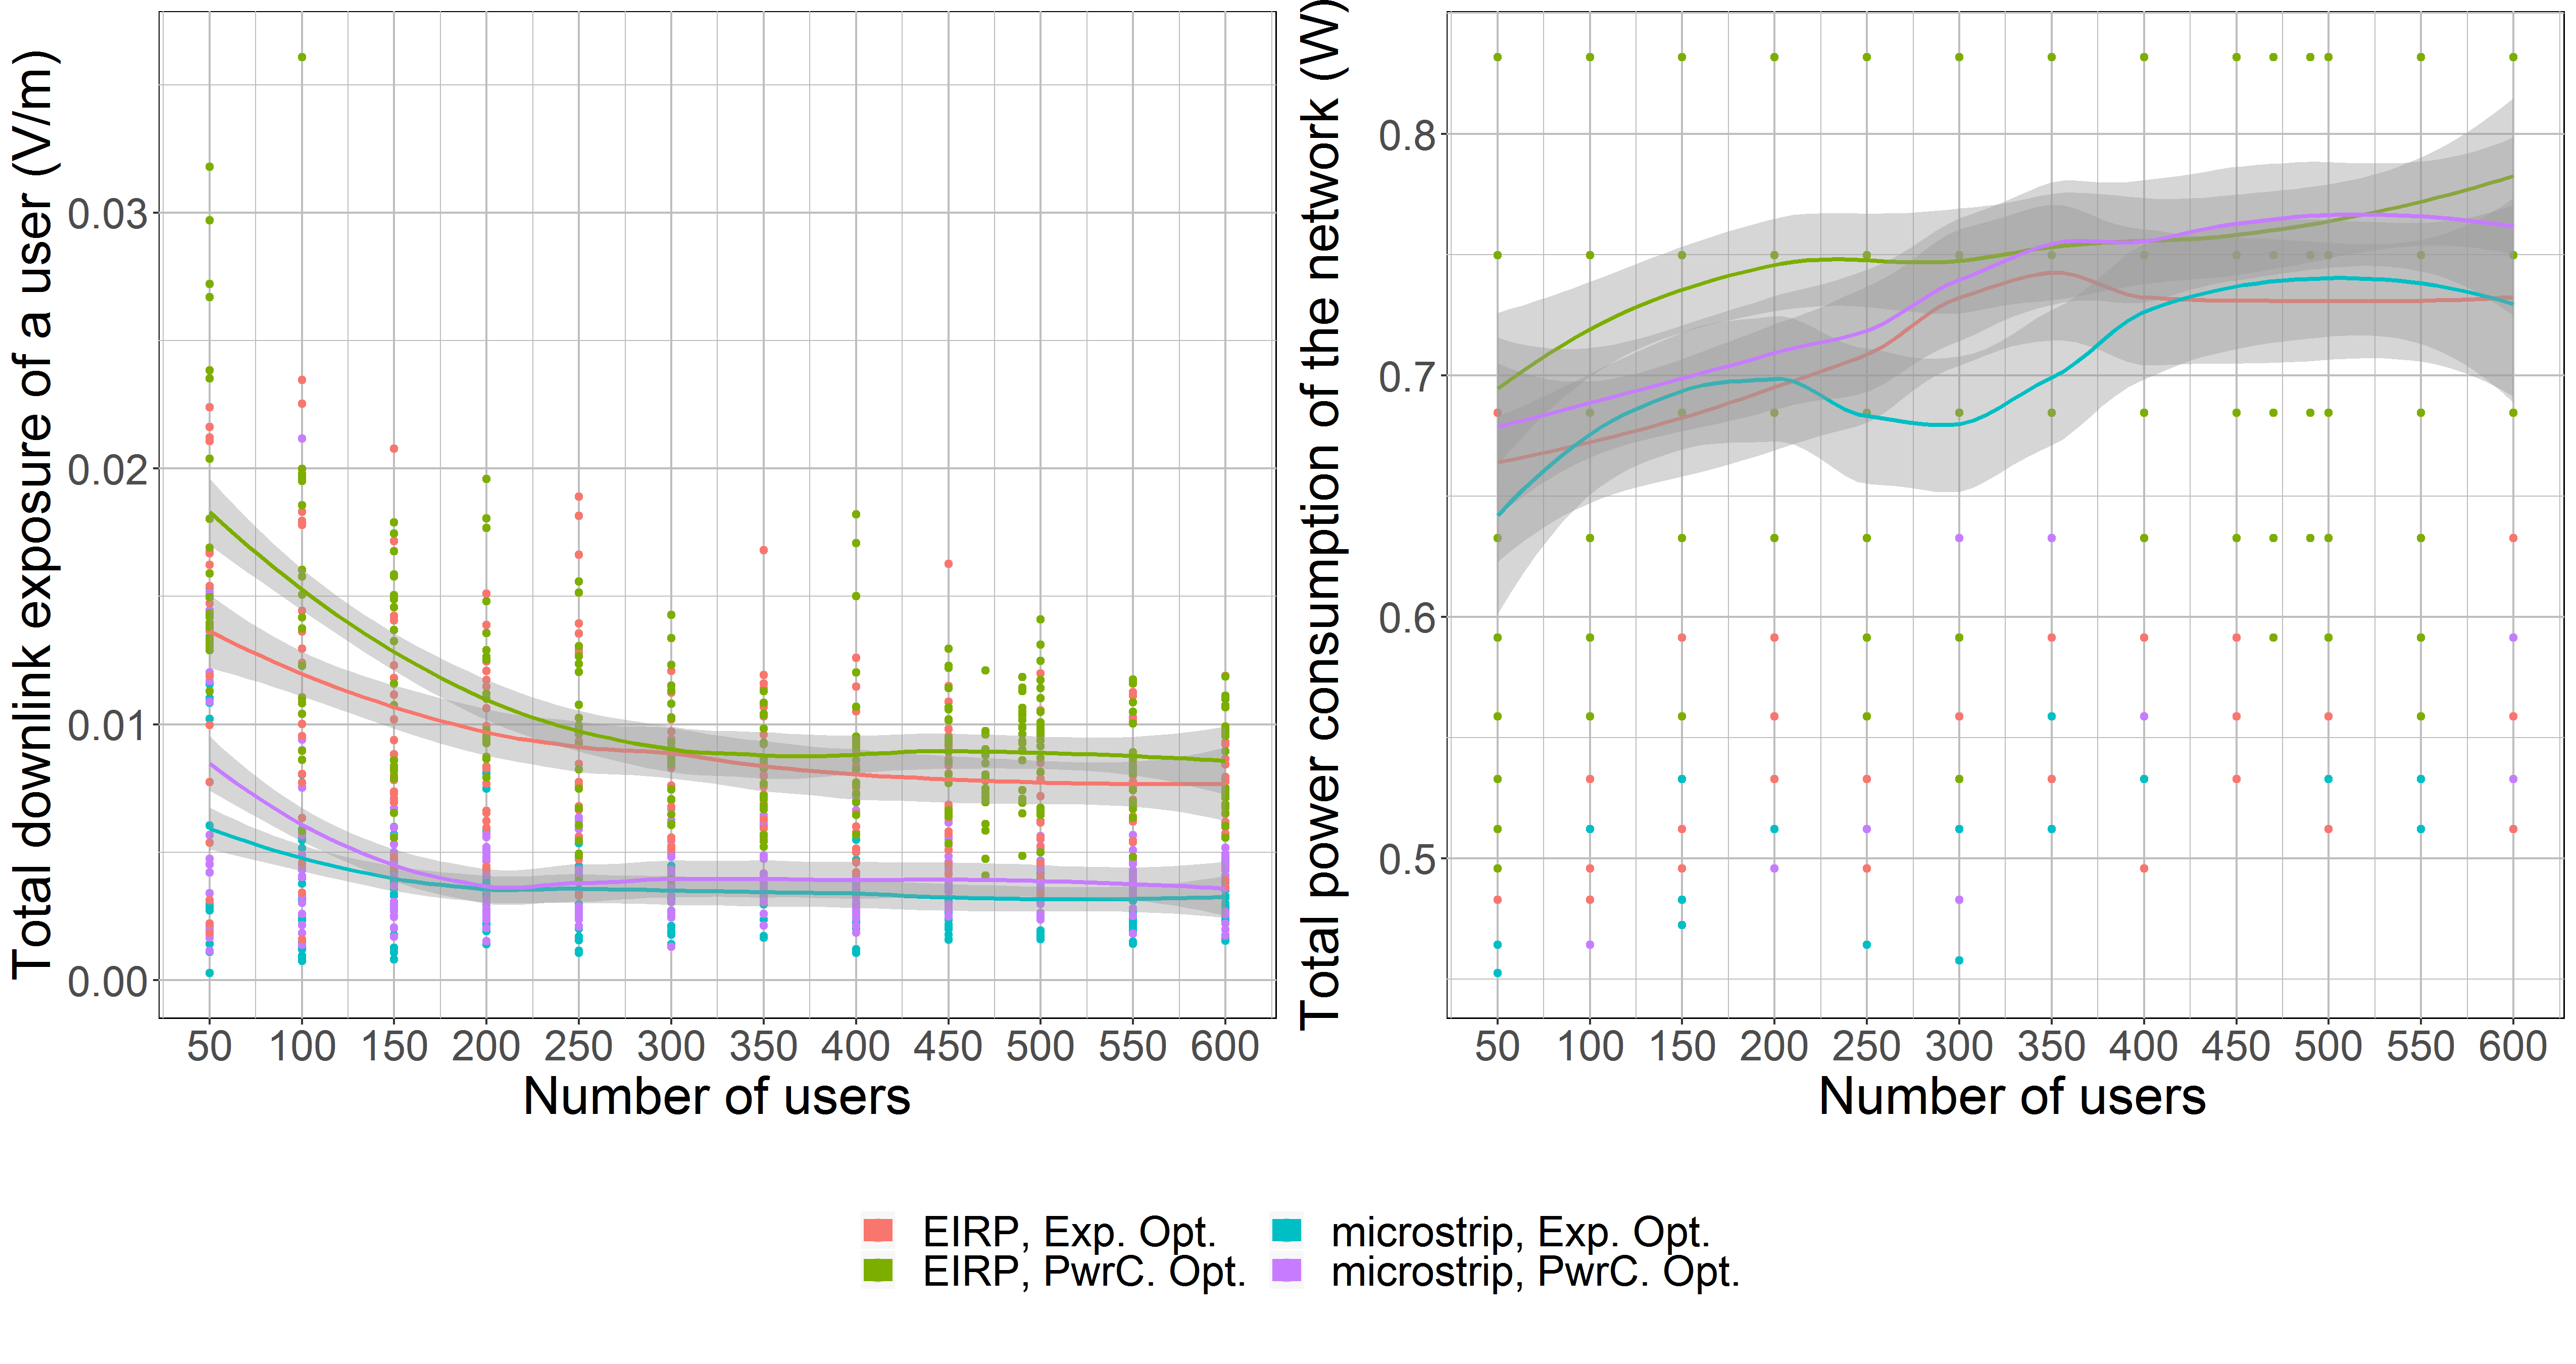
\includegraphics[width=\textwidth]{../results/s2/uvsdlAndPc.png}
  \caption{This figure shows how different sources are influenced by an increasing number of users. }
  \label{fig:s2b_dlAndPc}
\end{figure}

The downlink exposure is shown in figure \ref{fig:s2b_dlAndPc} on the left and is directly influenced by the percentage of covered users. 
The electromagnetic exposure decreases when more users become uncovered. Since an \gls{isotropicradiator} in a power consumption optimized network (green)
will have the highest coverage, also the \gls{DL} electromagnetic radiation from \gls{UABS}s will be highest compared to other configurations.
----> Todo, discuss PC

\textcolor{red}{It is important to notice that the optimization strategies only consider \gls{DL} exposure and power consumption.
However, how much radiation is absorbed by the users originating from all sources is shown in \ref{fig:s2uvssar} and the relative position of 
the four configurations do not differ compared to the \ref{fig:s2b_dlAndPc}. So an \gls{DL} exposure optimized network with an \gls{isotropicradiator}
 which result in the highest electromagnetic exposure for this scenario will also have the highest specific absorption rate according to figure
 \ref{fig:s2uvssar}. The same applies for the other configurations as well.}

\begin{figure}[h!]
  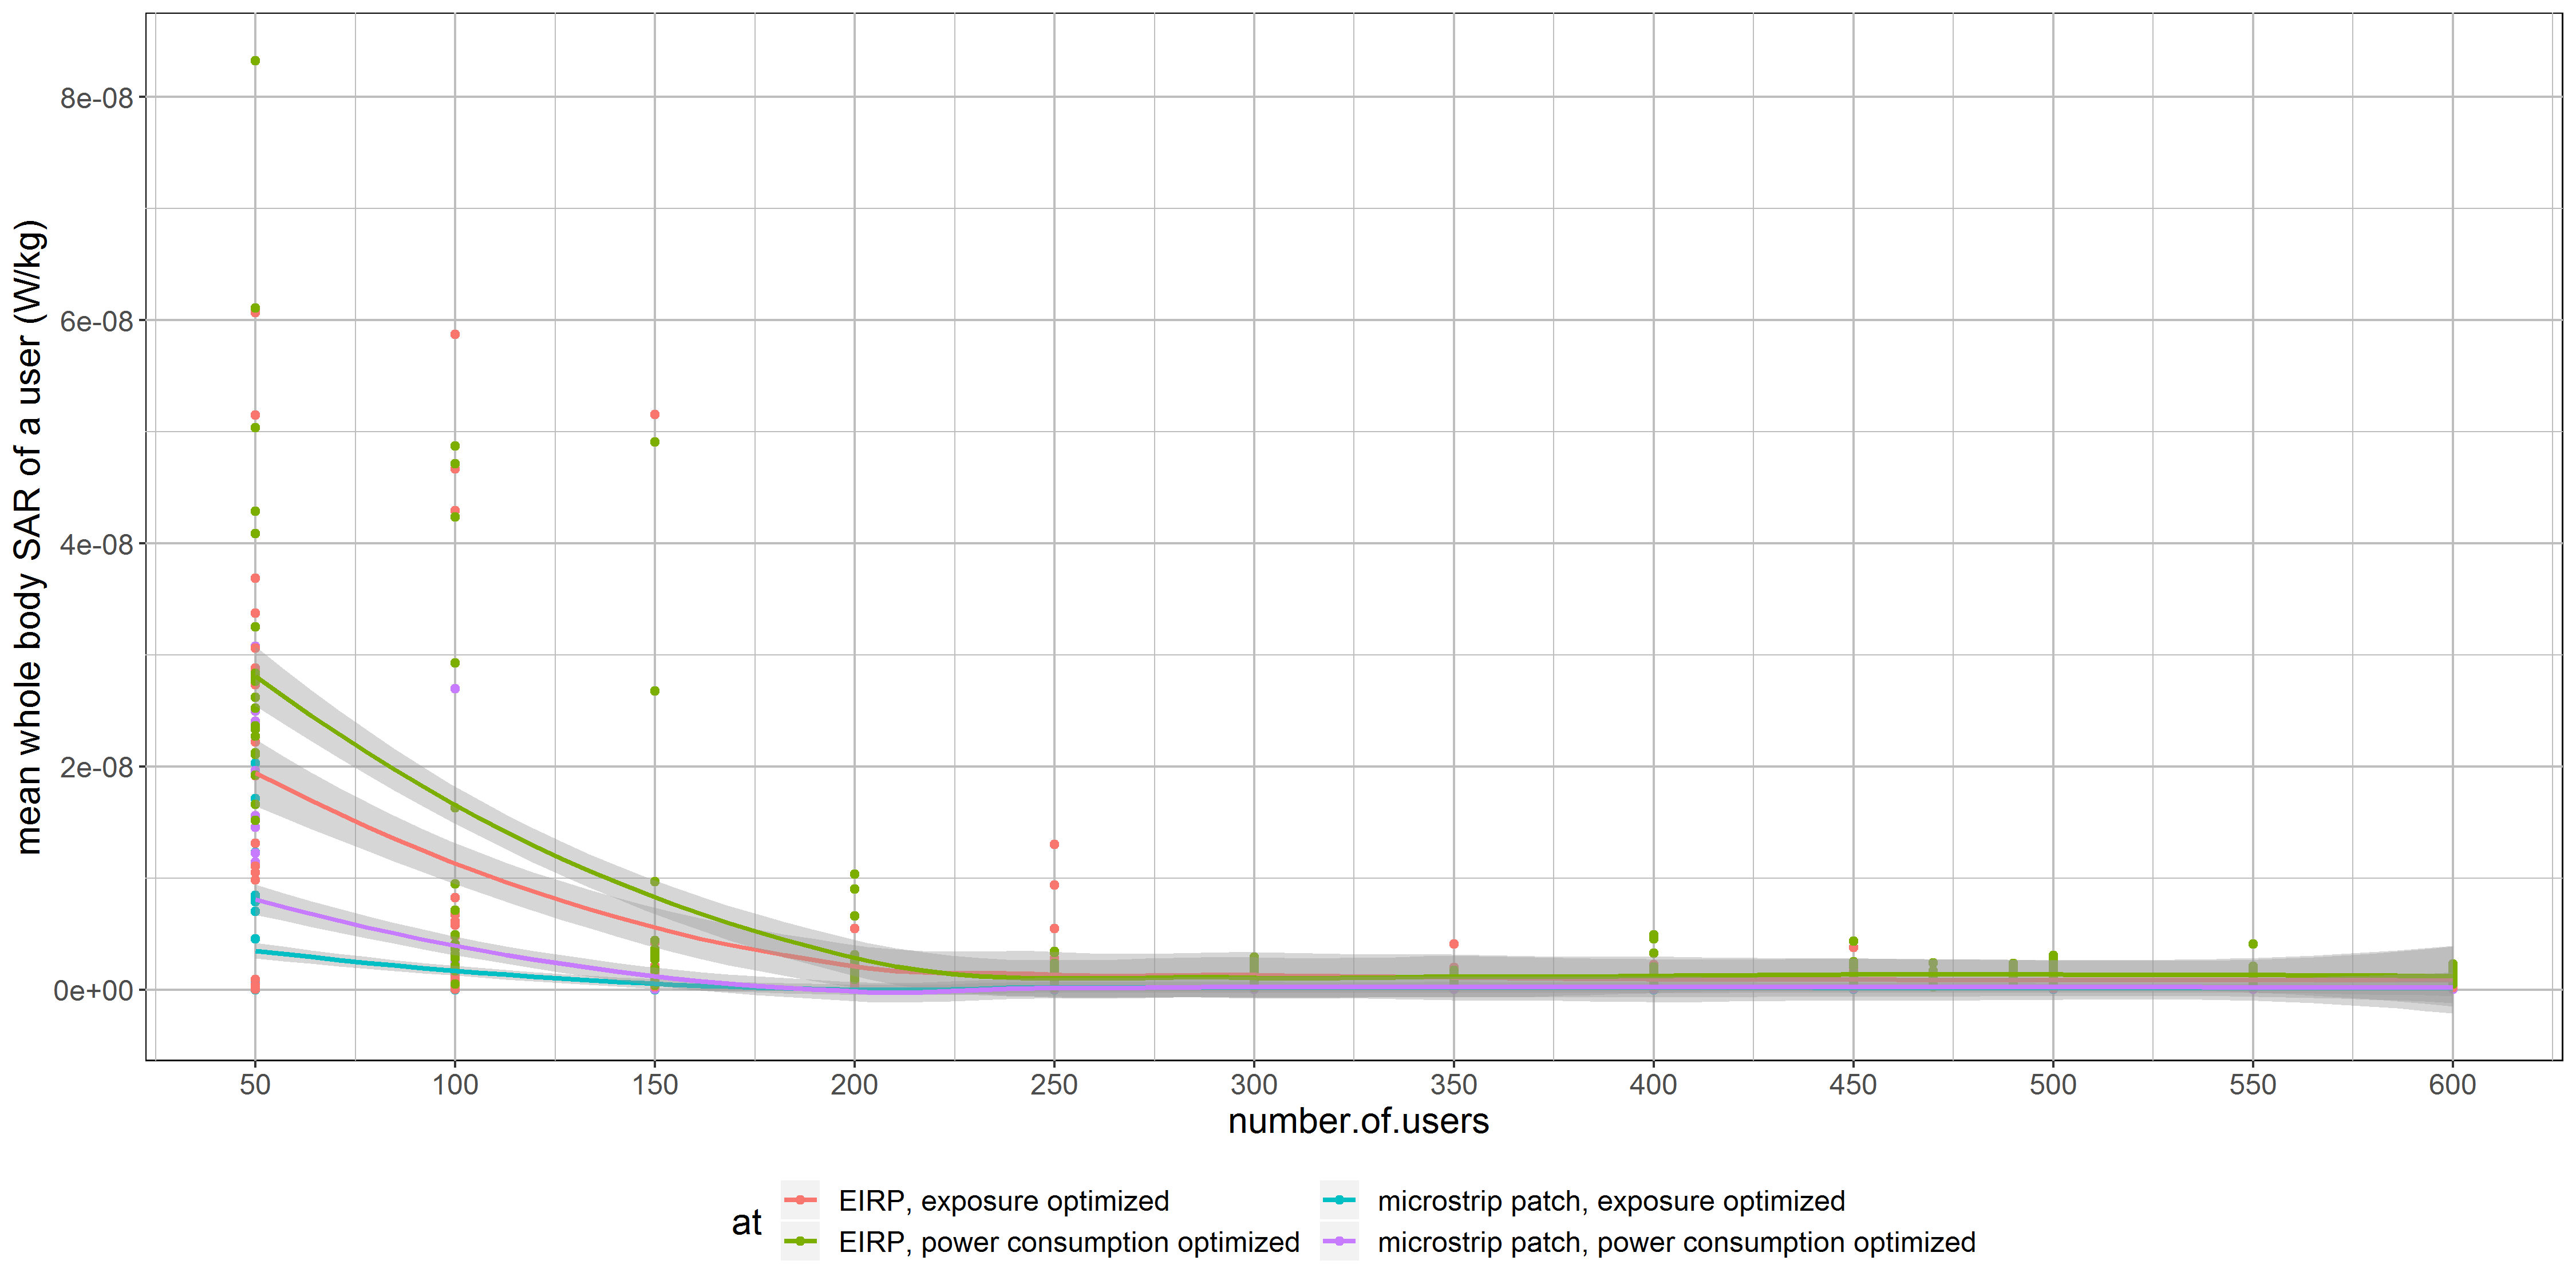
\includegraphics[width=\textwidth]{../results/s2/uvssar.png}
  \caption{This figure shows how different sources are influenced by an increasing number of users. }
  \label{fig:s2uvssar}
\end{figure}

Figure \ref{fig:s2fourSourcesMatrix} investigates the assets of each source to the total \gls{SAR}. All four 
configuration show that for 200 users and up, base stations are the main source of electromagnetic radiation.
For less users, the electromagnetic radiation from the user's device is the dominant factor. Figure \ref{fig:s2uvsnumcovusers} already 
showed that for 200 users and less, the number of covered user's is higher  but there is still only one \gls{UABS} available.
So \gls{UE}  need to radiate much more in order to still be able to reach that one drone.

The red line proves once again that the far field radiation from \gls{UE} can be neglected. The \gls{SAR} from 
neighbouring devices is not zero as it looks from figure \ref{fig:s2fourSourcesMatrix} but is just really low compared to the much higher
\gls{SAR}-values from other sources.

\begin{figure}[h!]
  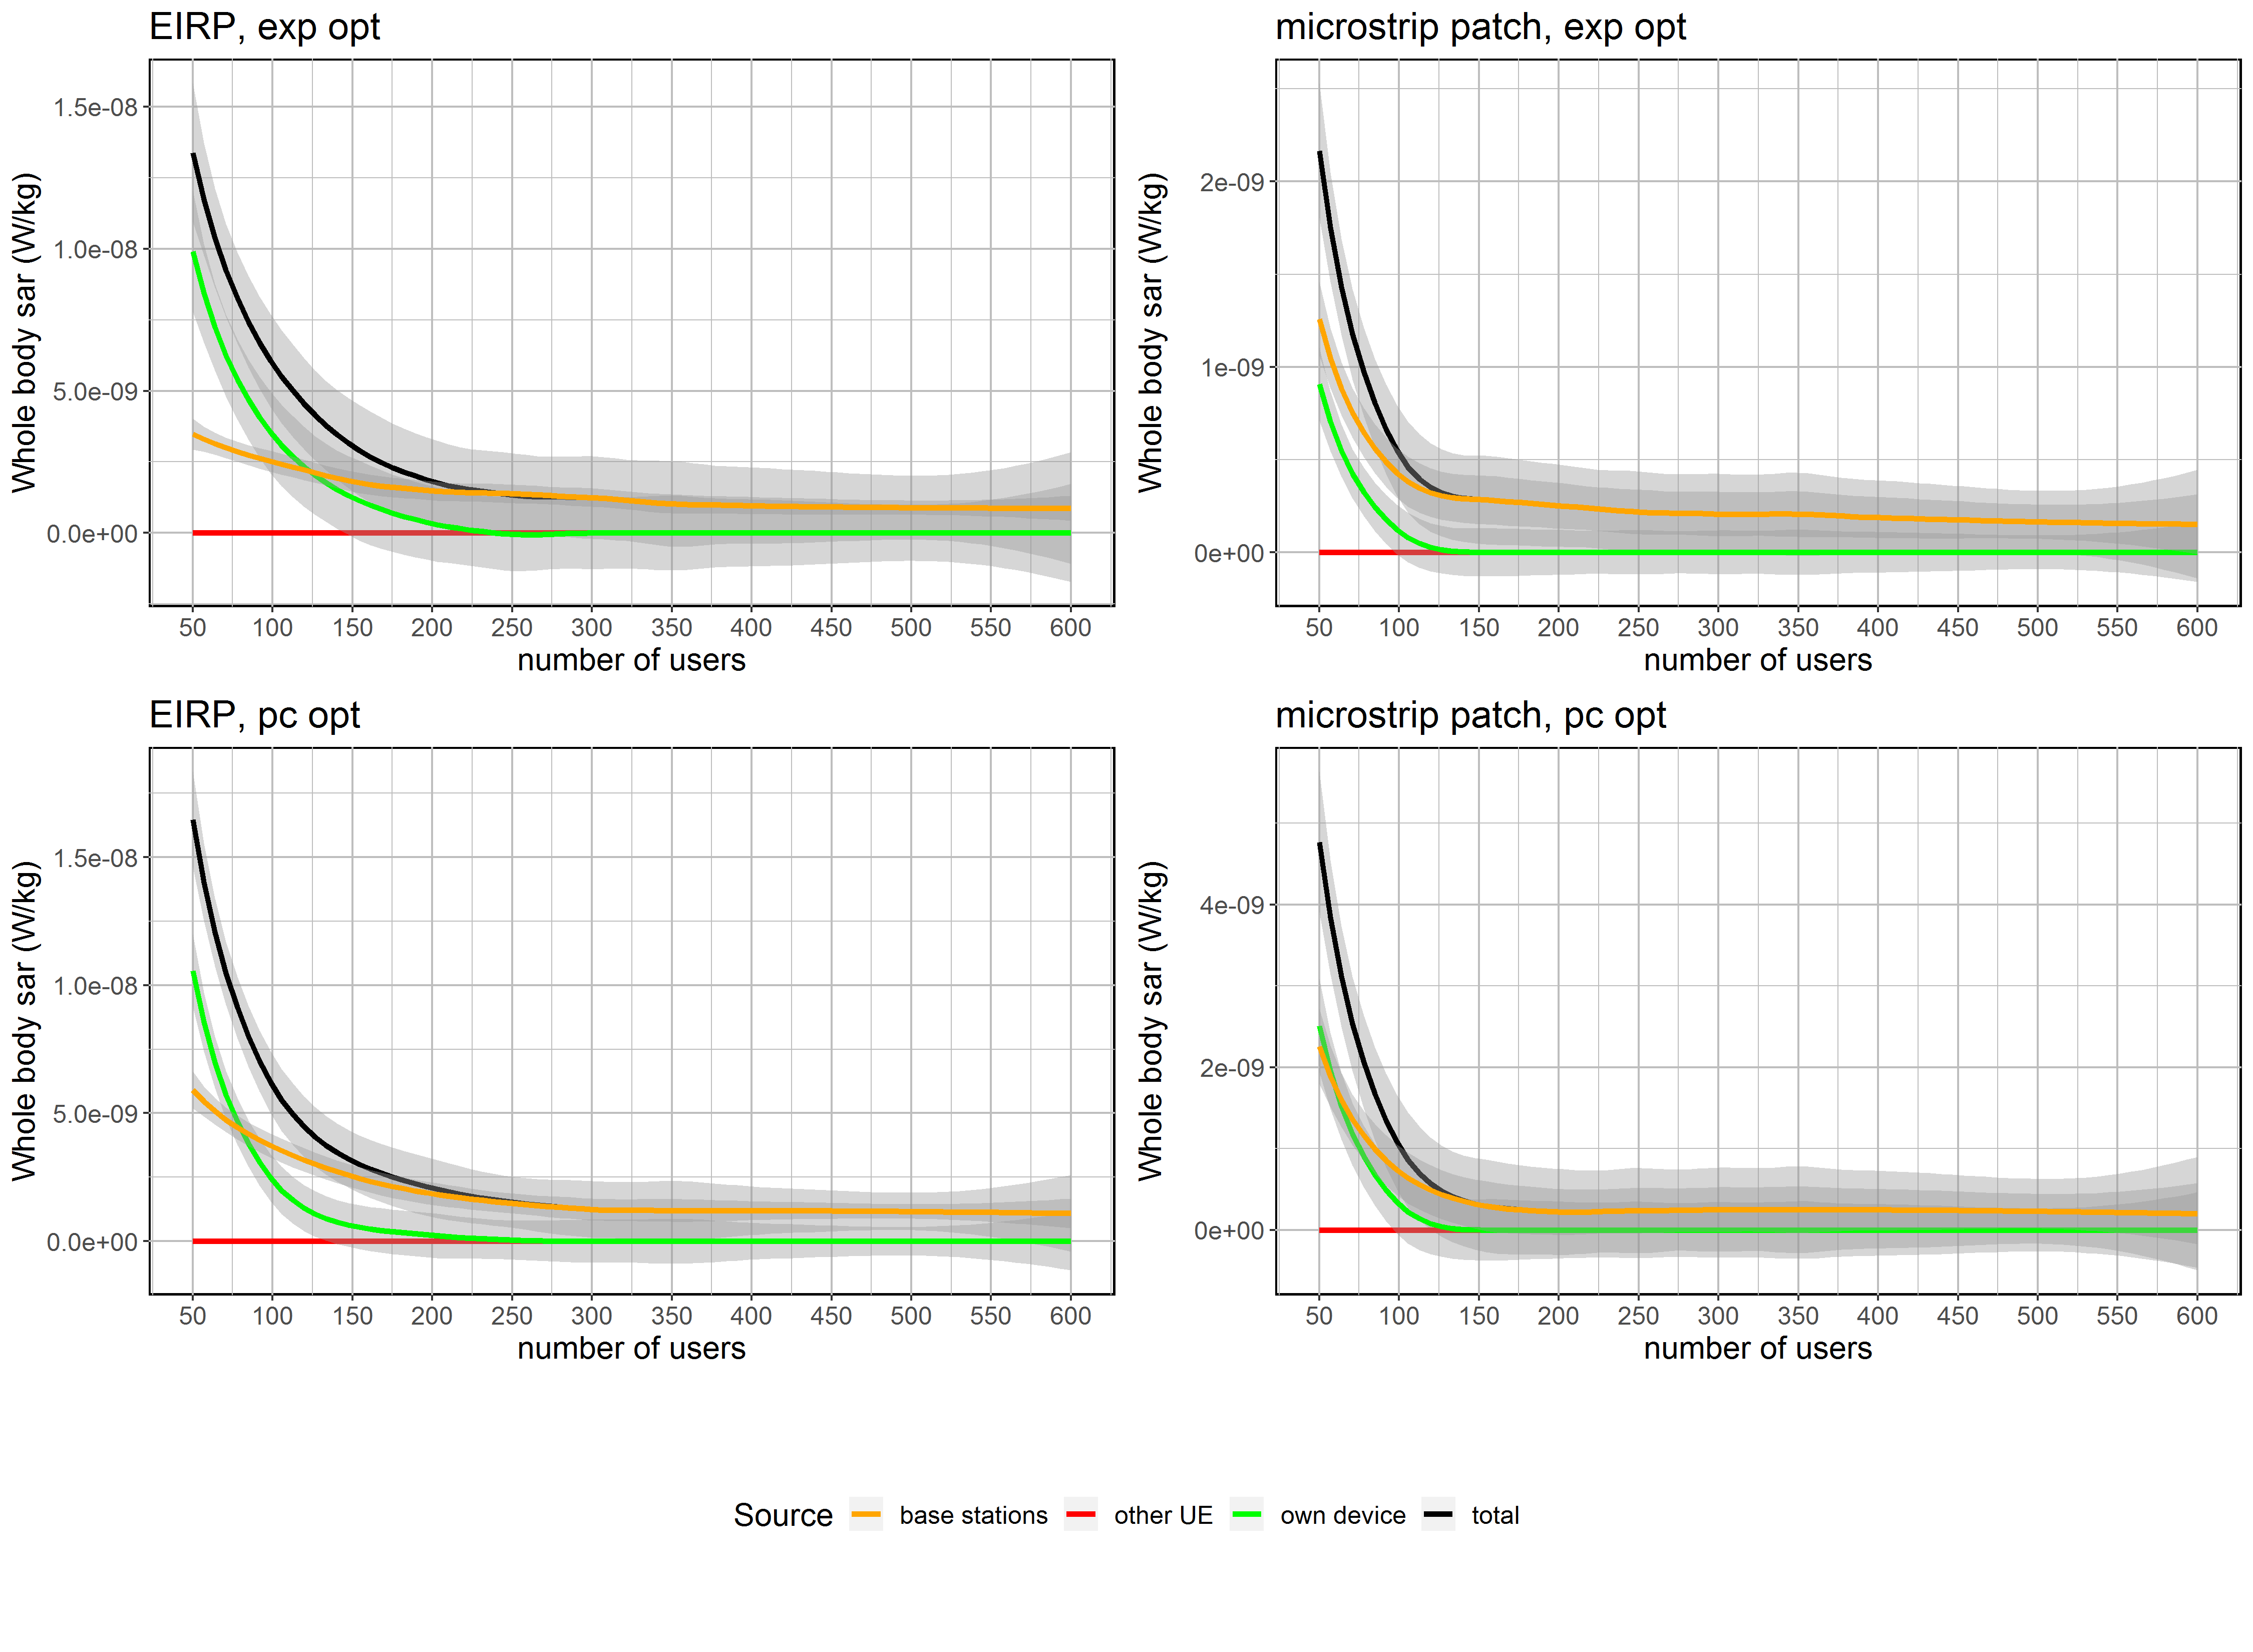
\includegraphics[width=\textwidth]{../results/s2/uFourSources.png}
  \caption{This figure shows how different sources are influenced by an increasing number of users. }
  \label{fig:s2fourSourcesMatrix}
\end{figure}

%%%%%%%%%%%%%%%%%%%%%%%%%%%%%%%%%%%%%%%%%%%%%%%%%%%%%%%%%%%%%%%%%%%%%%%%%%%%%%%%%%%%%%%%%%%%%%%%%%%%%%%%%%%%%s
\section{Scenario 3: Unlimited Drones}
\label{s3}

This scenario has just like the previous scenario much more users in the network 
and investigates the same cases including the variable flying height and the variable number of  users.
The only difference is that the restriction of only one \gls{UABS}s is dropped.

\subsection{Influence of the Flying Altitude}
\label{S3A}

The first case of this scenario examines how the network behaves for various flying heights and a fixed number of 224 users.
Scenario 2 already explained that when only one drone is available, a power consumption optimized network won’t result in a low 
powered network. In this scenario, there is no limitation on the number of drones and the network remains thus unaltered after the decision 
algorithm is done. Figure \ref{fig:s3a_dlAndPc} clearly proves that the different optimization strategies are correctly applied by 
the decision algorithm and work as intended.
Power consumption optimized networks have indeed a lower power consumption but therefore results in higher electromagnetic radiation.
In contrast to an exposure optimized network that, as expected, will reduce the electromagnetic exposure by using more drones and thence also increasing the network's power consumption.

\begin{figure}[h!]
  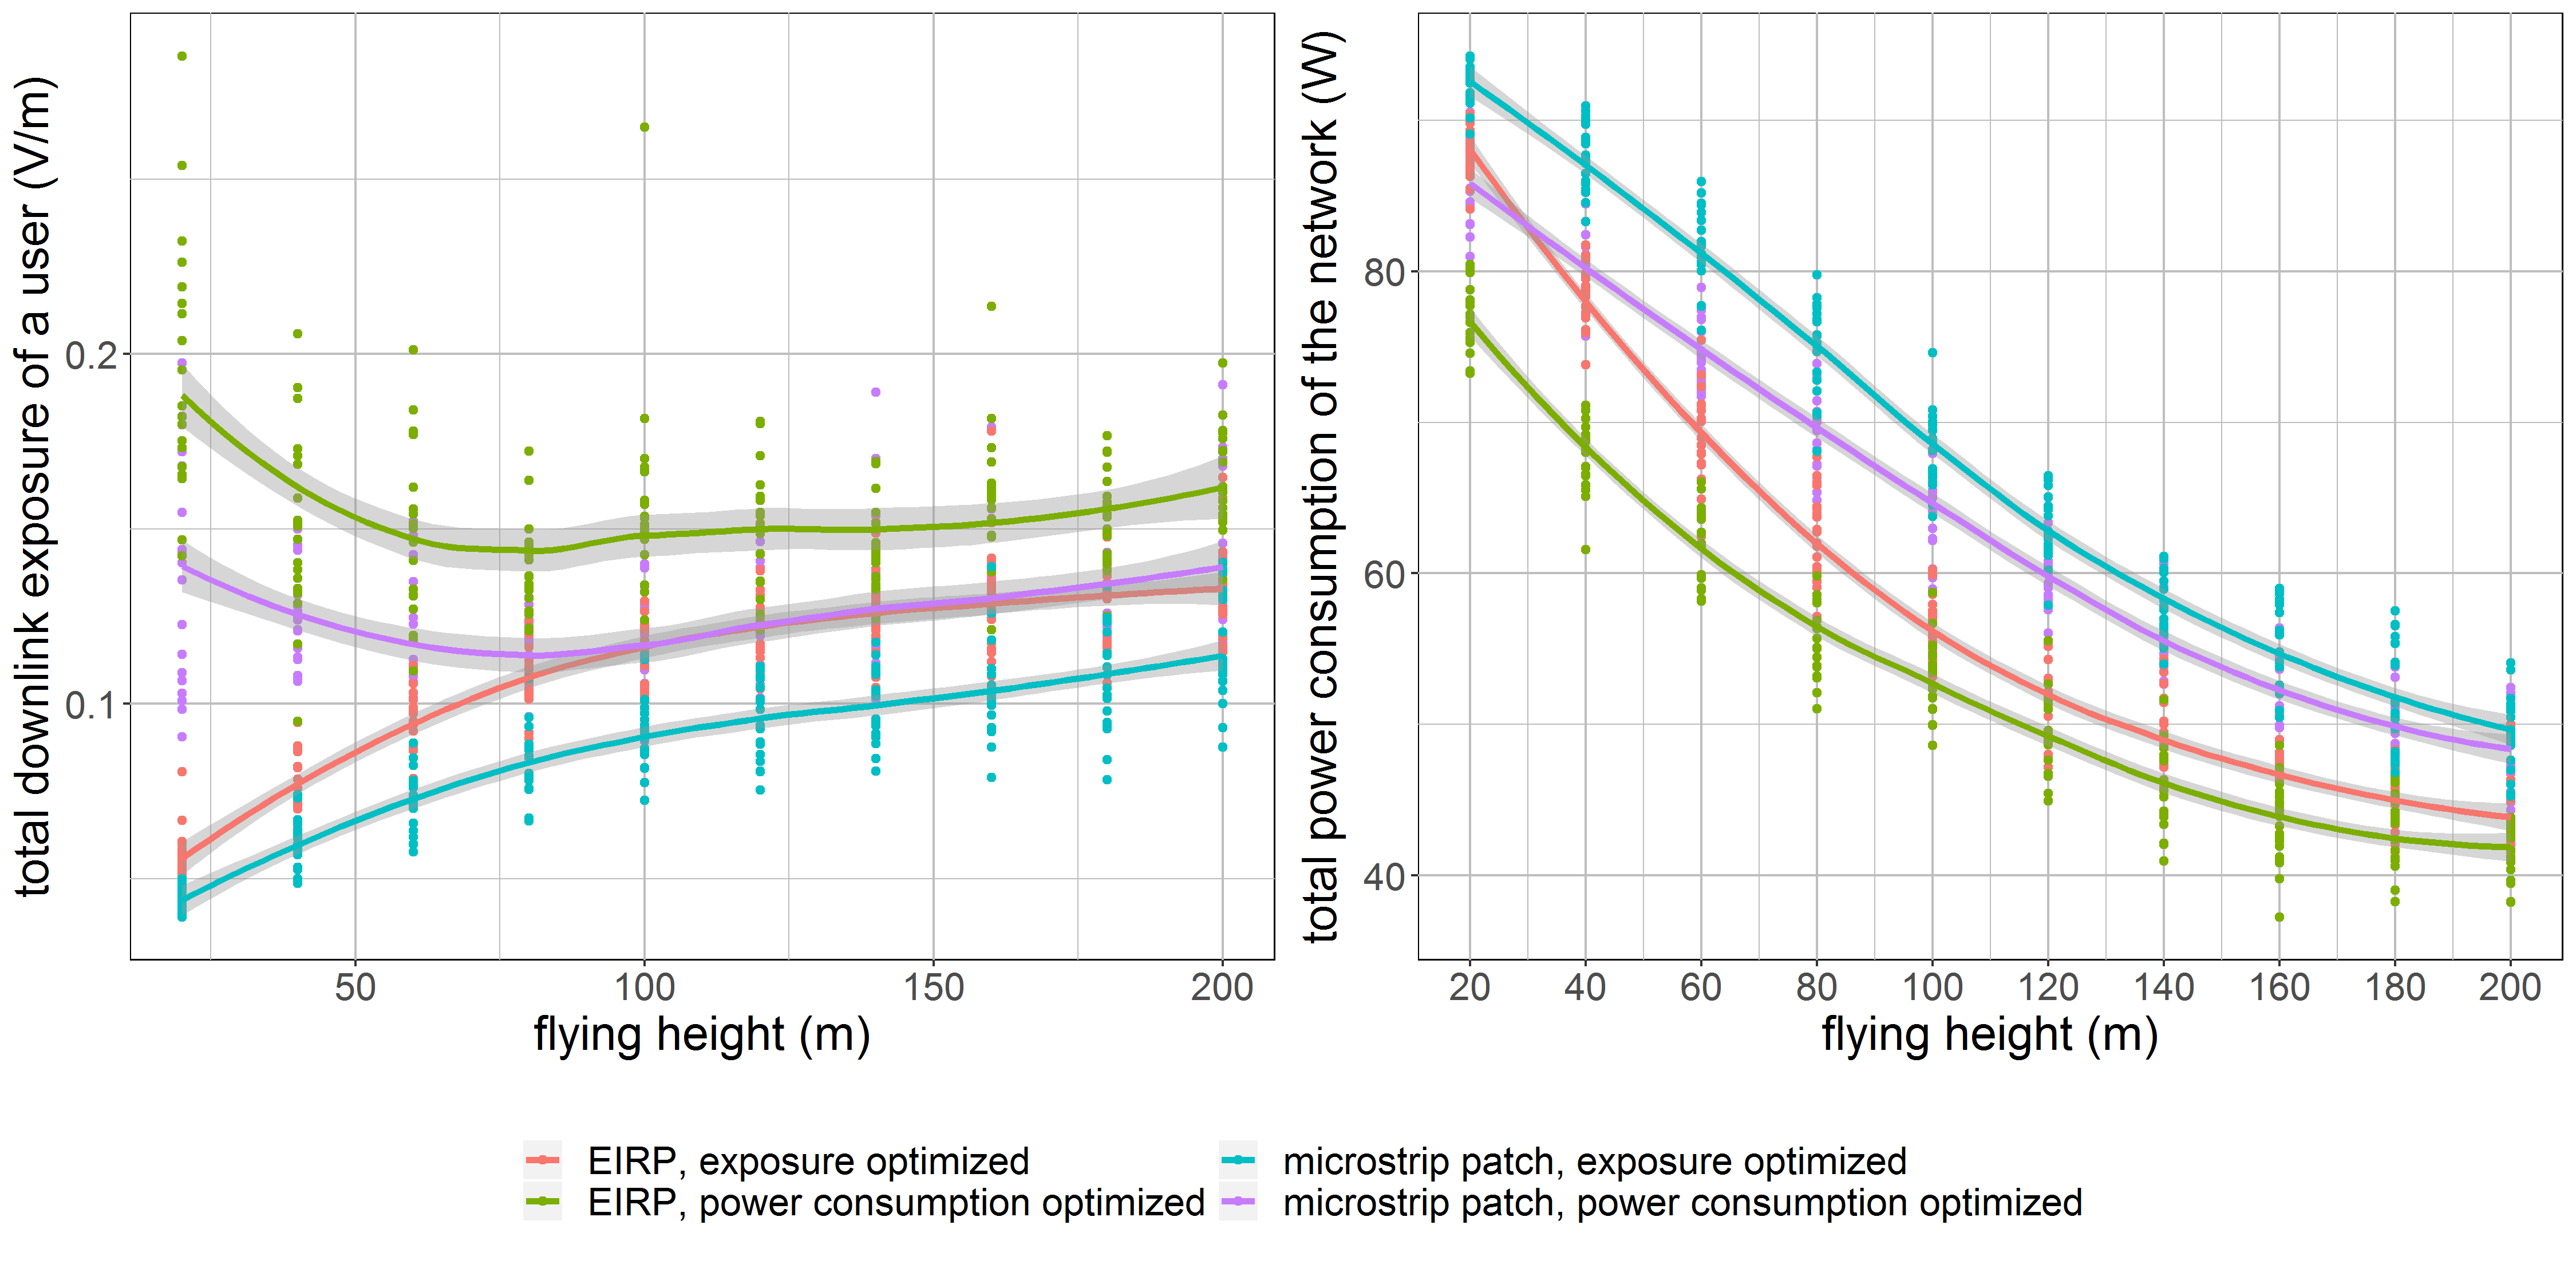
\includegraphics[width=\textwidth]{../results/s3/fhvsdlAndPc.png}
  \caption{The influence of the flying height on the downlink electromagnetic radiation of the average user.. This graph shows the percentage of covered users by one drone for different flying heights.}
  \label{fig:s3a_dlAndPc}
\end{figure}

The difference in optimization strategy is clearly bigger for low flying drones. The exposure in a power consumption  optimized network starts high and 
decreases while an exposure optimized network behaves the opposite. This can be explained when looking at figure \ref{fig:s3a_numDronesAndCov}.
At a flying height of 20 metres, the exposure optimized network has on average 220 to 224 \gls{UABS}s. That is (almost) one \gls{UABS} for each user
so it's logical that the electromagnetic exposure is very low.
The number of drones in a power consumption optimized network is much less in order to save energy but the tool still tries to reach for a 100\% coverage. Since 
there is a high path loss from obstructing buildings, \gls{UABS}s need to radiate much more to compensate for this. The exposure will thus be much higher for 
users in \gls{LOS}. This path loss reduces when the \gls{UABS}s start to fly higher then the average  building and therefore decreases exposure.
Also the exposure optimized network profits from the advantage of higher flying drones. Much less drones are required for only a little bit more 
electromagnetic exposure.

\begin{figure}[]
  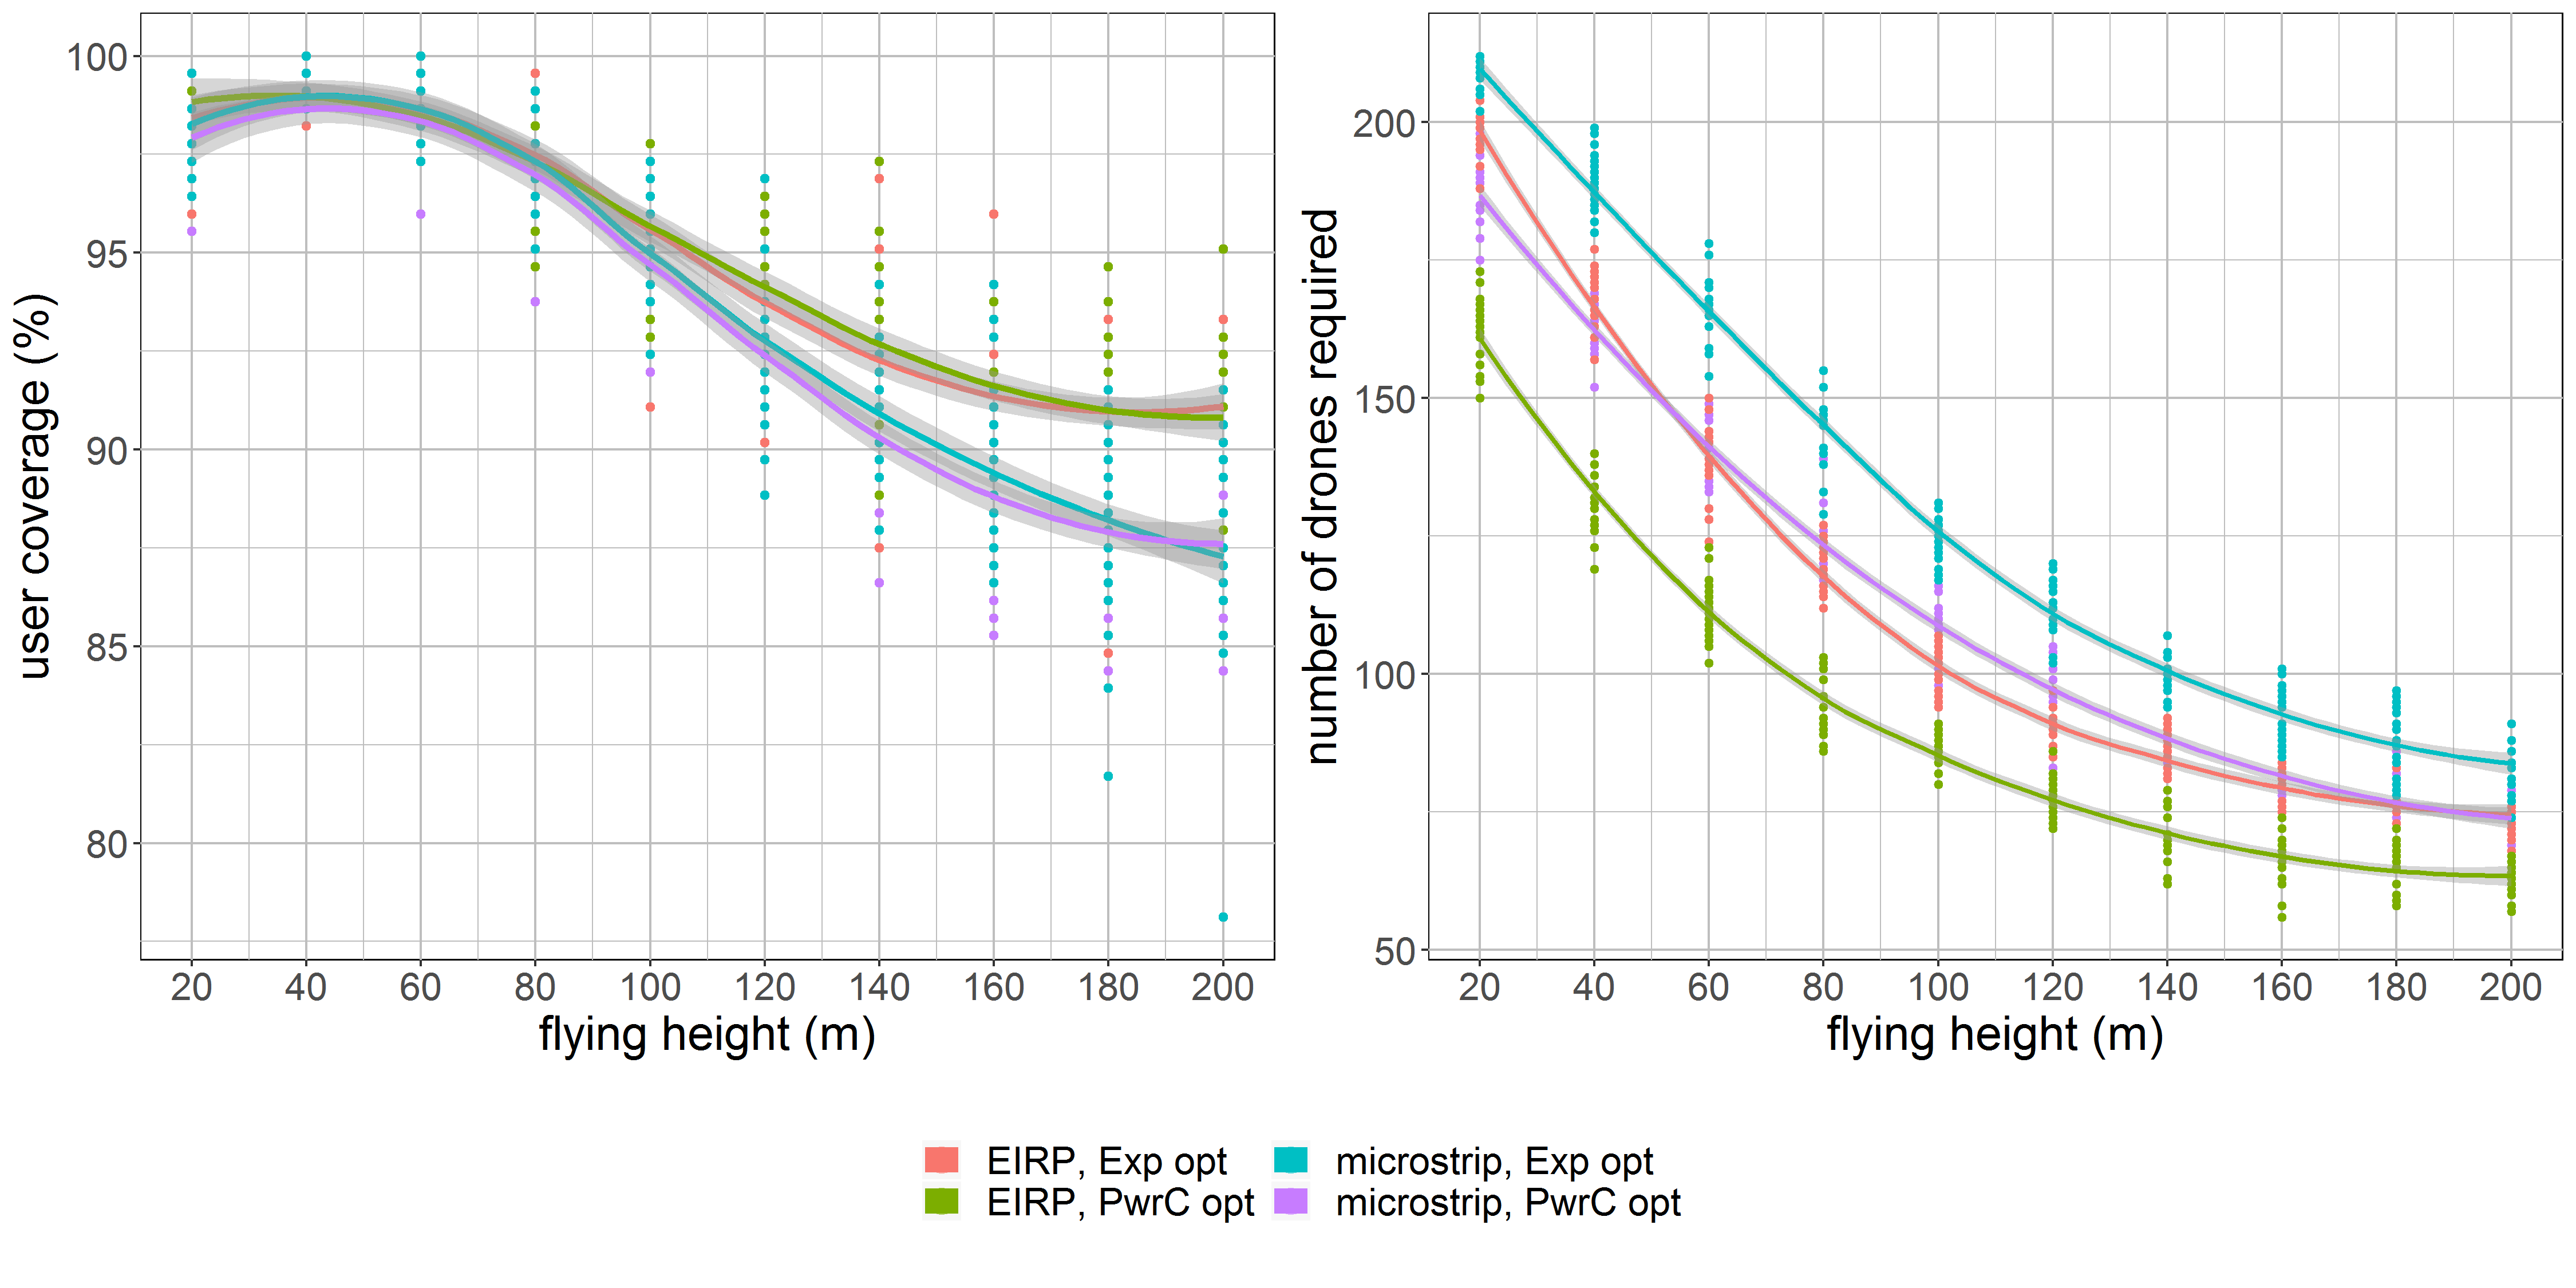
\includegraphics[width=\textwidth]{../results/s3/fhvsnumdronesAndCov.png}
  \caption{This graph shows how much drones are required for different flying heights while trying to achieve a 100\% coverage.}
  \label{fig:s3a_numDronesAndCov}
\end{figure}

Both \ref{fig:s3a_numDronesAndCov} and \ref{fig:s3a_dlAndPc} show that the network profit from increasing the flying altitude. 
Not only less drones are needed but also the power consumption is lower. Both can be explained by the lower path loss when \gls{UABS}s fly higher.

Scenario 1 already proved that with low flying drones, the main source of electromagnetic radiation are \gls{UABS}. 
This changed around 80 meters where \gls{UL} electromagnetic radiation of the \gls{UE}
 exceeds \gls{DL} radiation in order to still be able to reach the high flying \gls{UABS}s. We know from 
 previous scenarios that the behaviour of the \gls{SAR} behave very similar to the downlink exposure \ref{fig:s3a_sar}.

\begin{figure}[]
  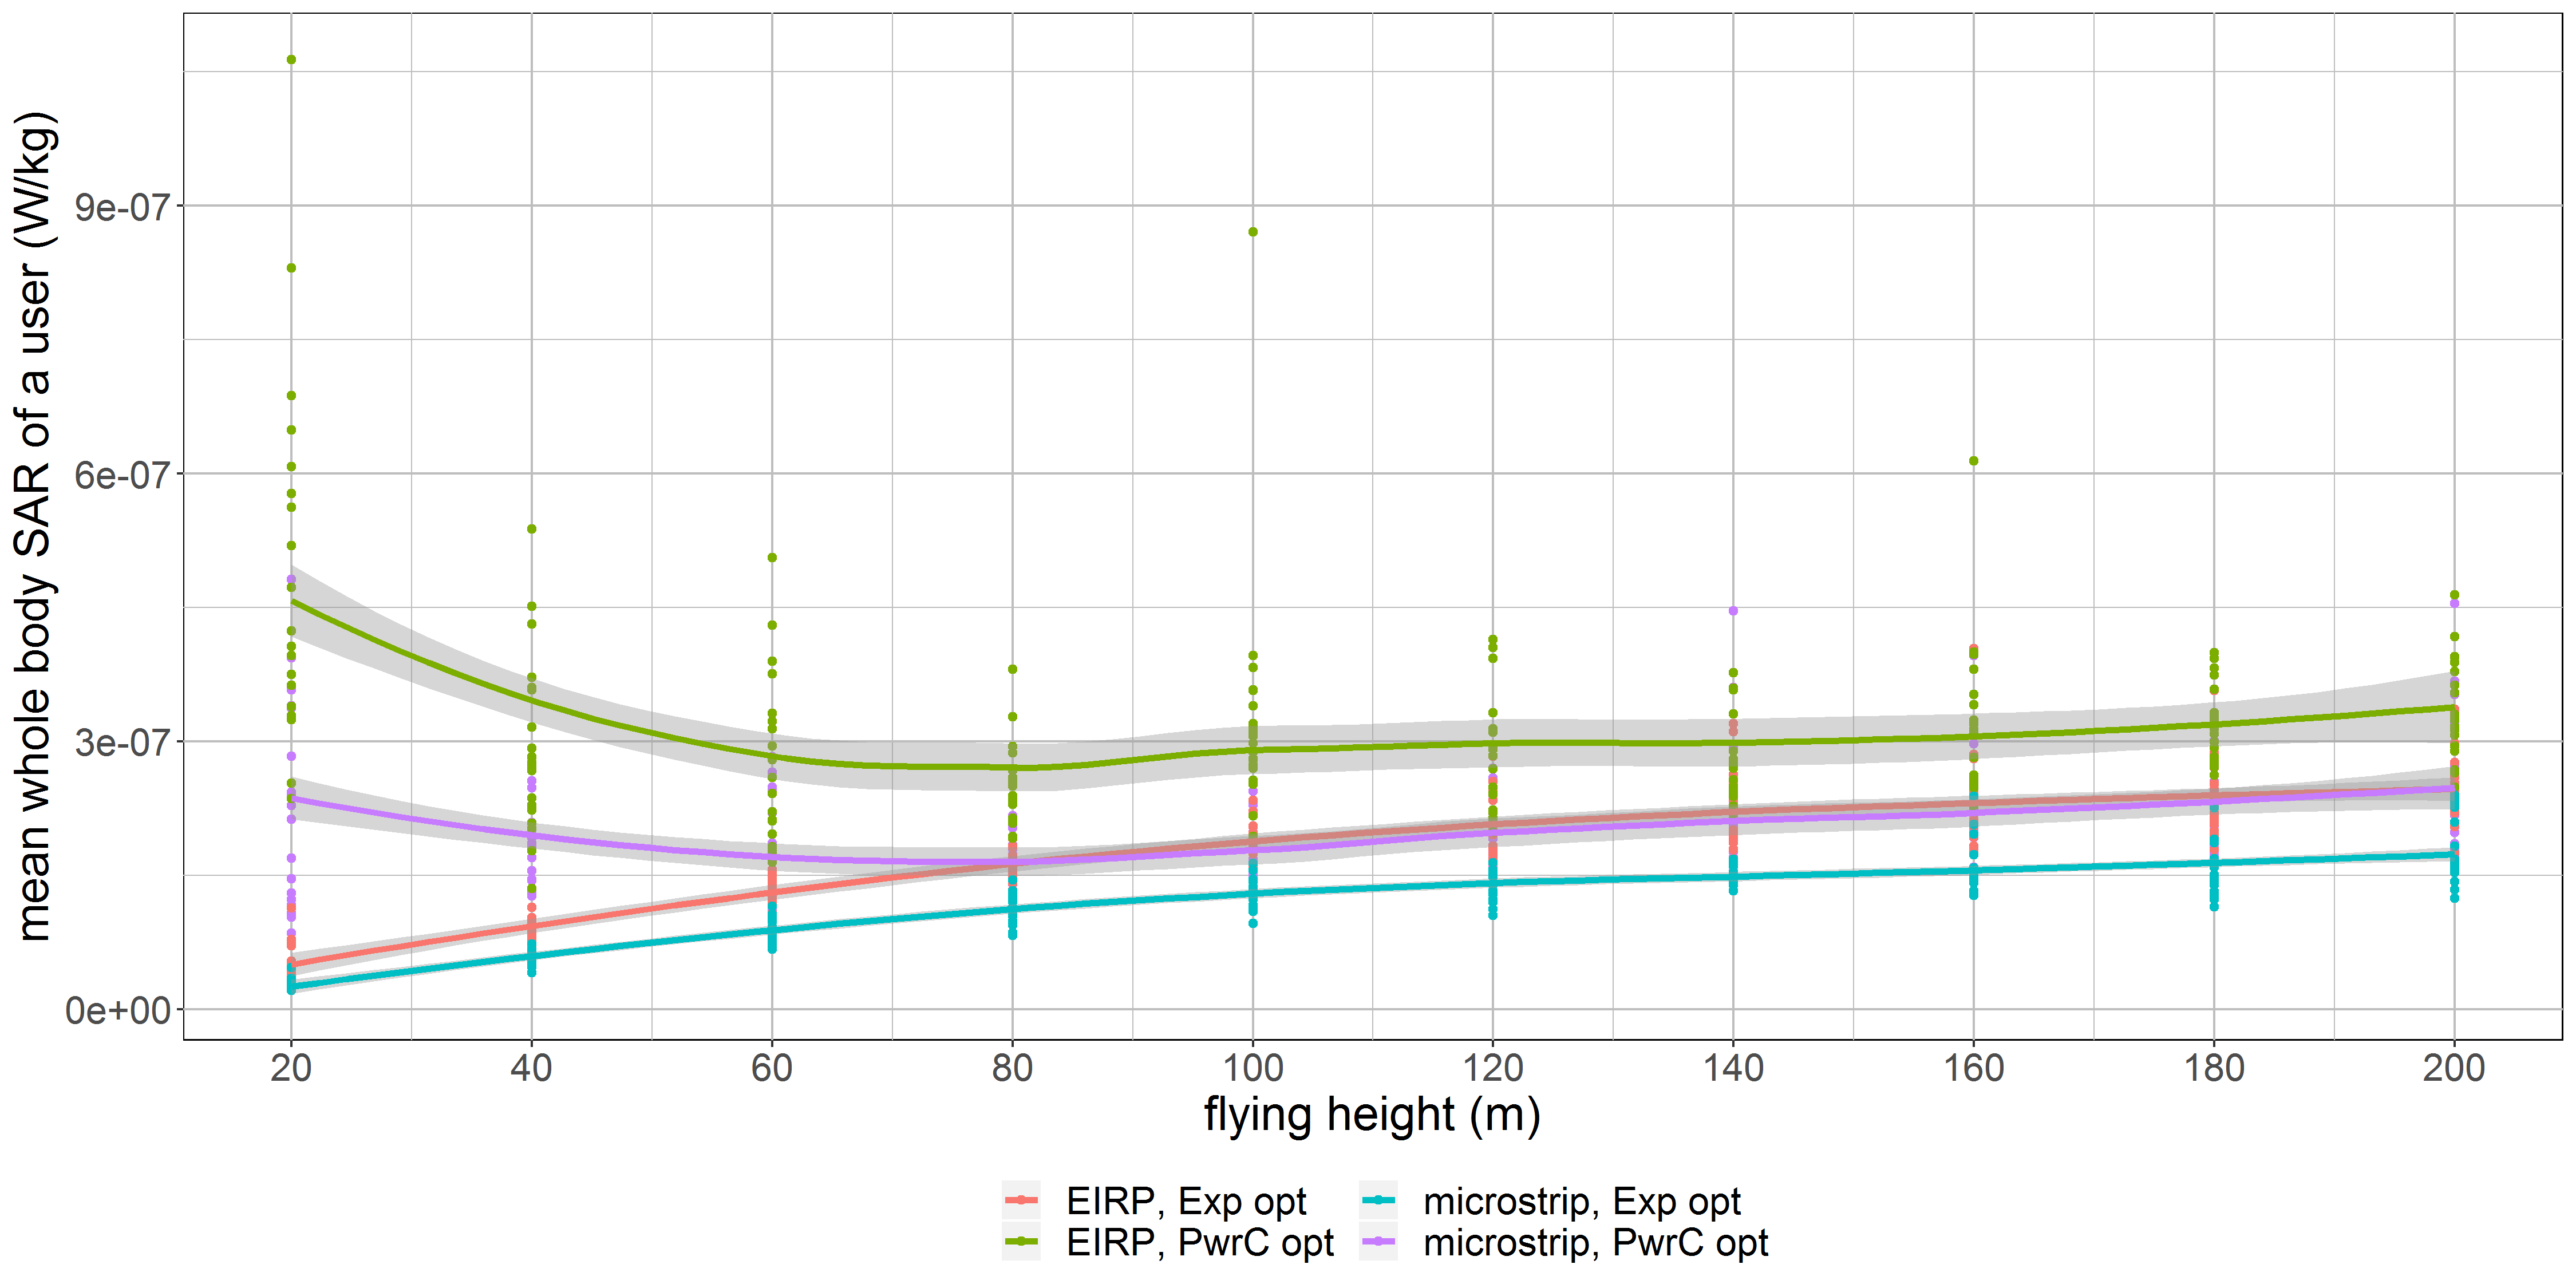
\includegraphics[width=\textwidth]{../results/s3/fhvssar.png}
  \caption{The influence of the flying height on the weighted average $SAR_{10g}$ of users in the network.}
  \label{fig:s3a_sar}
\end{figure}

When looking at the different individual sources in \ref{fig:s3a_fourSourcesMatrix}, we see 
that $SAR_{10g}^{ul}$ is logarithmic increasing despite the fact that figure \ref{fig:s1_fhsar} showed that the $SAR_{10g}^{ul}$
increases exponentially. This was however deducted when only one user is present in the network as opposed to this scenario 
where 224 users are present. The covered users will still behave like in scenario 1 but fig. \ref{fig:s3a_numDronesAndCov} 
shows also that less users will be covered when flying altitude increases. The average $SAR_{10g}^{ul}$ is thus somewhere in the middle.
This theory is also supported by the fact that the $SAR_{10g}^{ul}$ in an microstrip patch antenna is less in figurer \ref{fig:s3a_fourSourcesMatrix} 
and the percentage of covered users is also less \ref{fig:s3a_numDronesAndCov}

\begin{figure}[]
  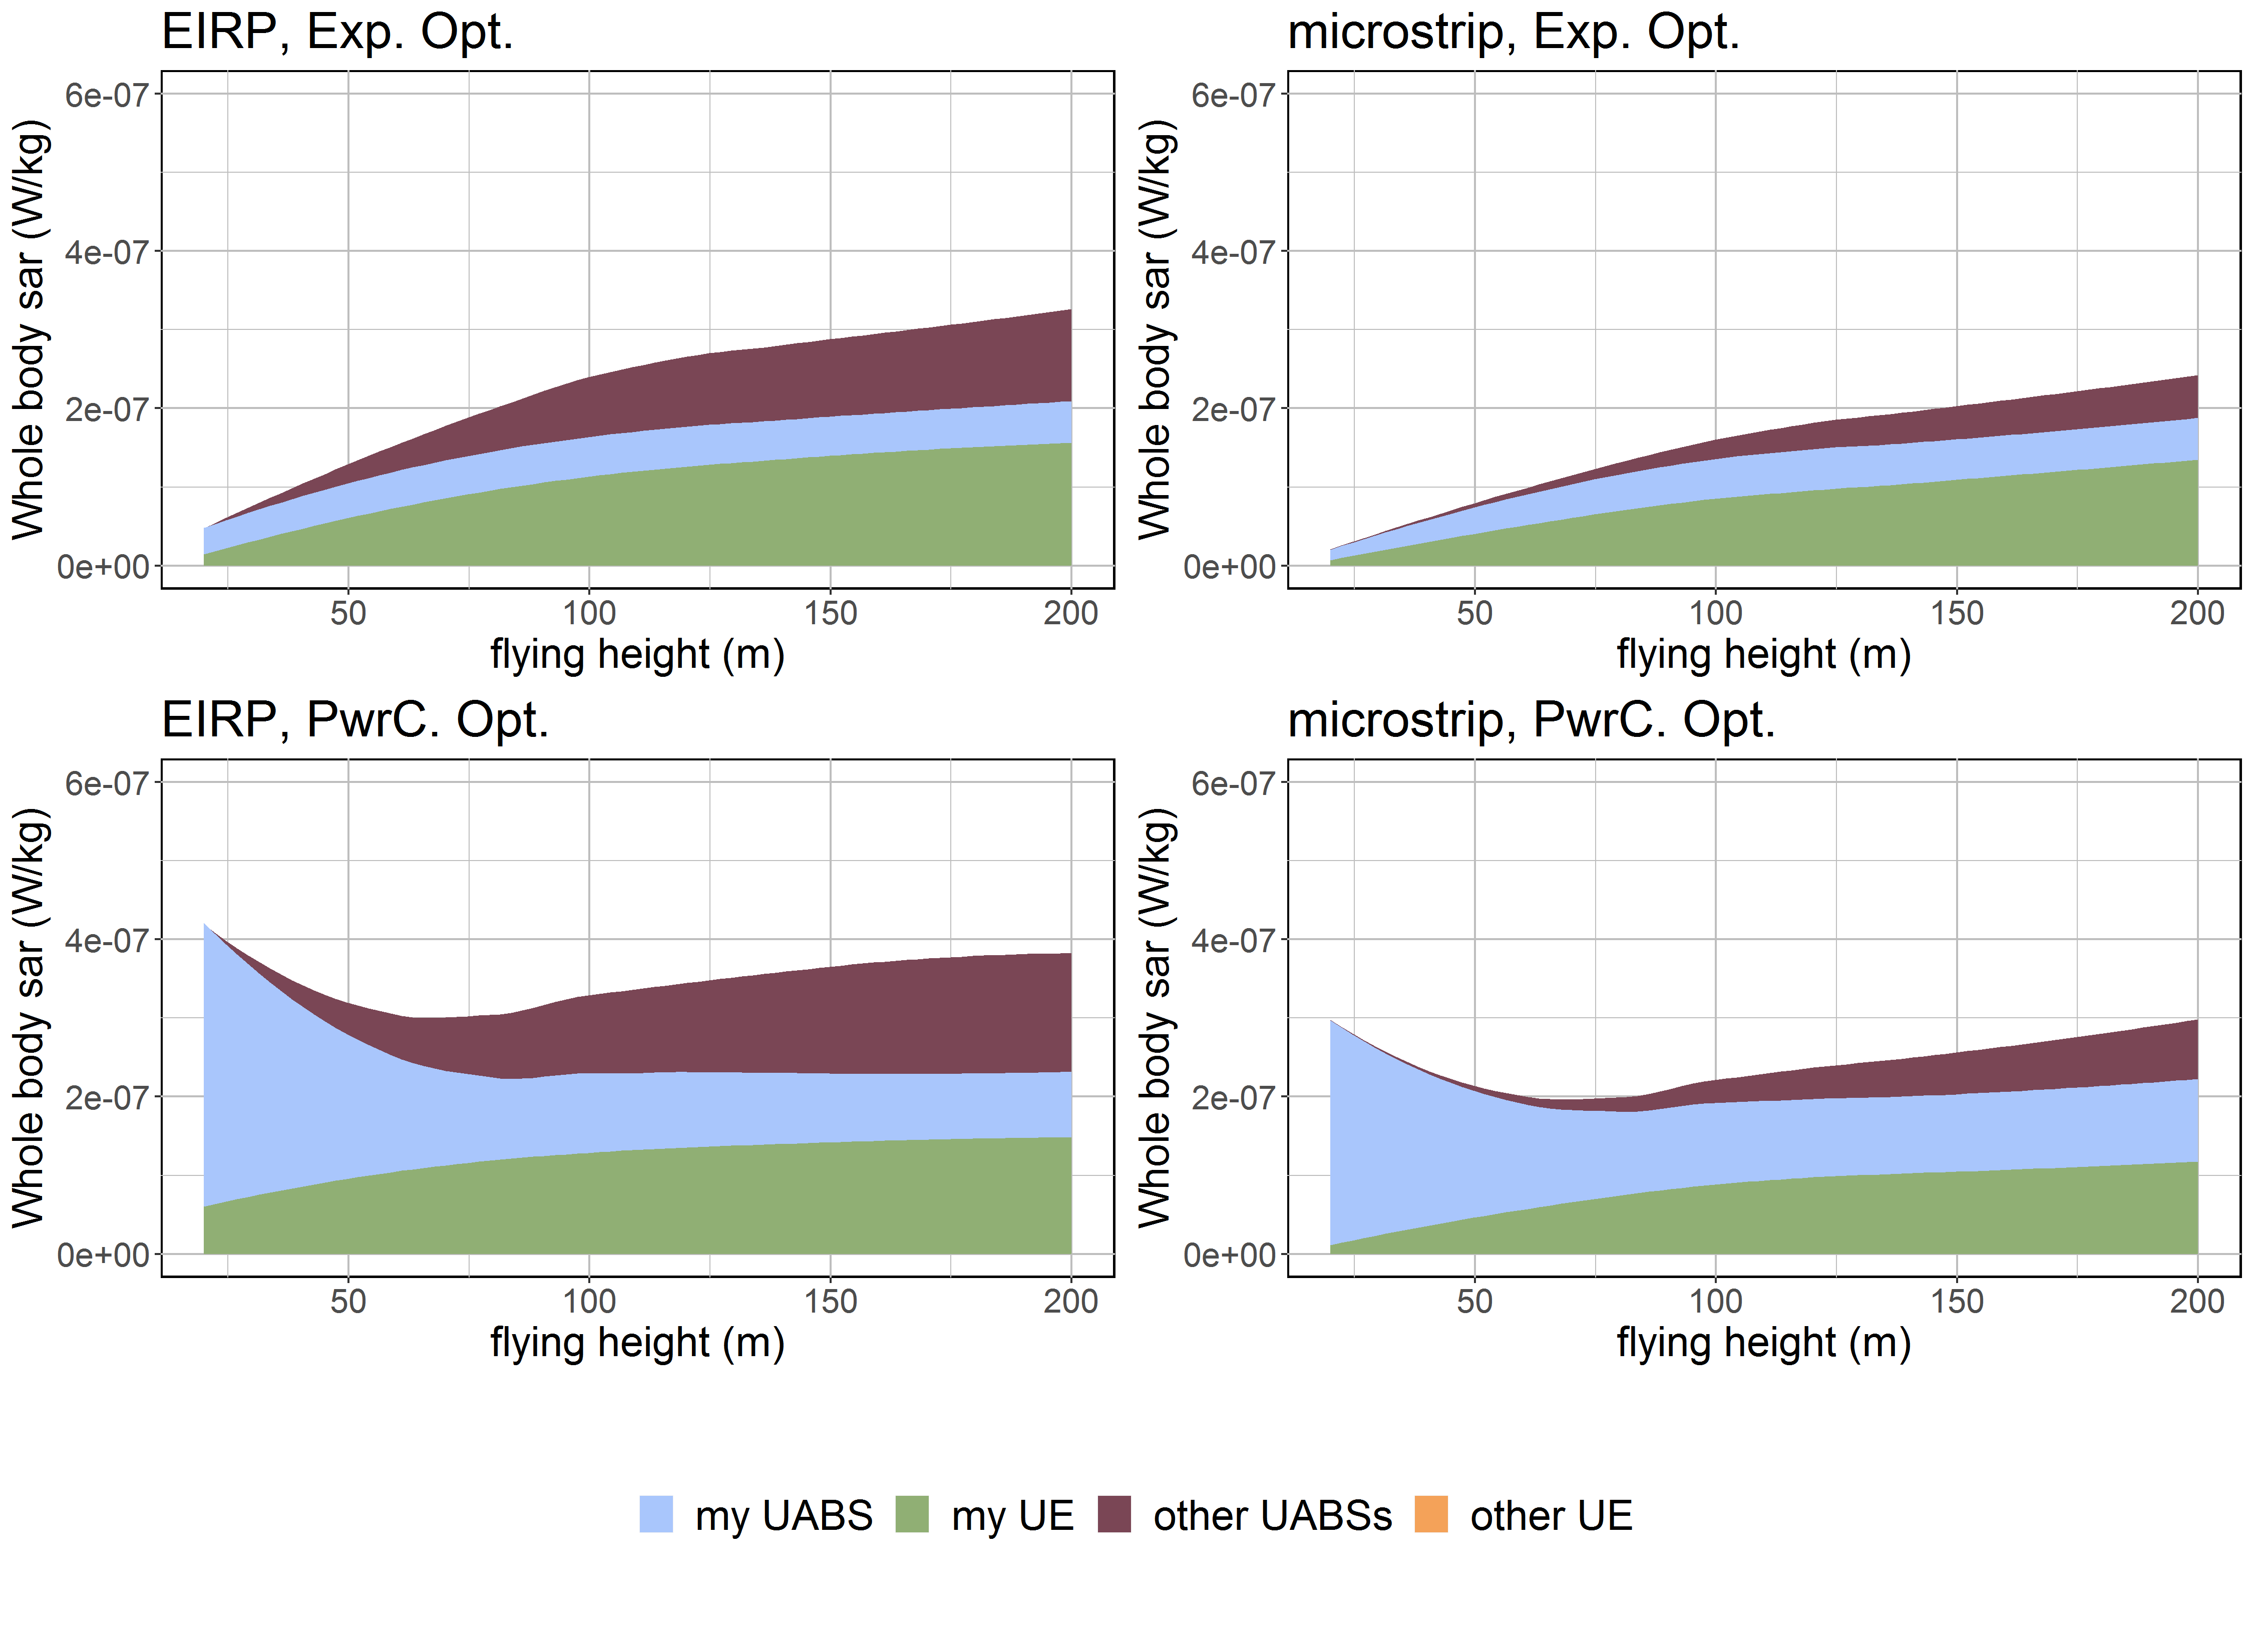
\includegraphics[width=\textwidth]{../results/s3/fhFourSources.png}
  \caption{Four Sources}
  \label{fig:s3a_fourSourcesMatrix}
\end{figure}

%%%%%%%%%%%%%%%%%%%%%%%%%%%%%%%%%%%%%%%%%%%%%%%%%%%%%%%%%%%%%%%%%%%%%%%%%%%%%
\FloatBarrier
\subsection{Influence of the number of users}
\label{S3B}

The last case of scenario 3 investigates variable number of users for a fixed flying height of 100 m. There is no 
restriction on the number of available drones just like in the previous case meaning that there are at most 
as much drones as users in the network. The correct behaviour of the decision algorithm became already clear in the previous subsection \ref{S3A}. 
Also this case proves this.

Figure \ref{fig:s3b_numDronesAndCov} shows on the left how the tool tries to reach a 100\% coverage. The tool reaches this goal 
better for larger populations. The difference remains however very little. The tool also requires more drones for these large 
populations which is a logical consequence of scenario \ref{s2b} where the percentage of covered users decreases for these larger populations.
 The difference in optimization strategy is very little for small amounts of people but increases very fast. 

\begin{figure}[h!]
  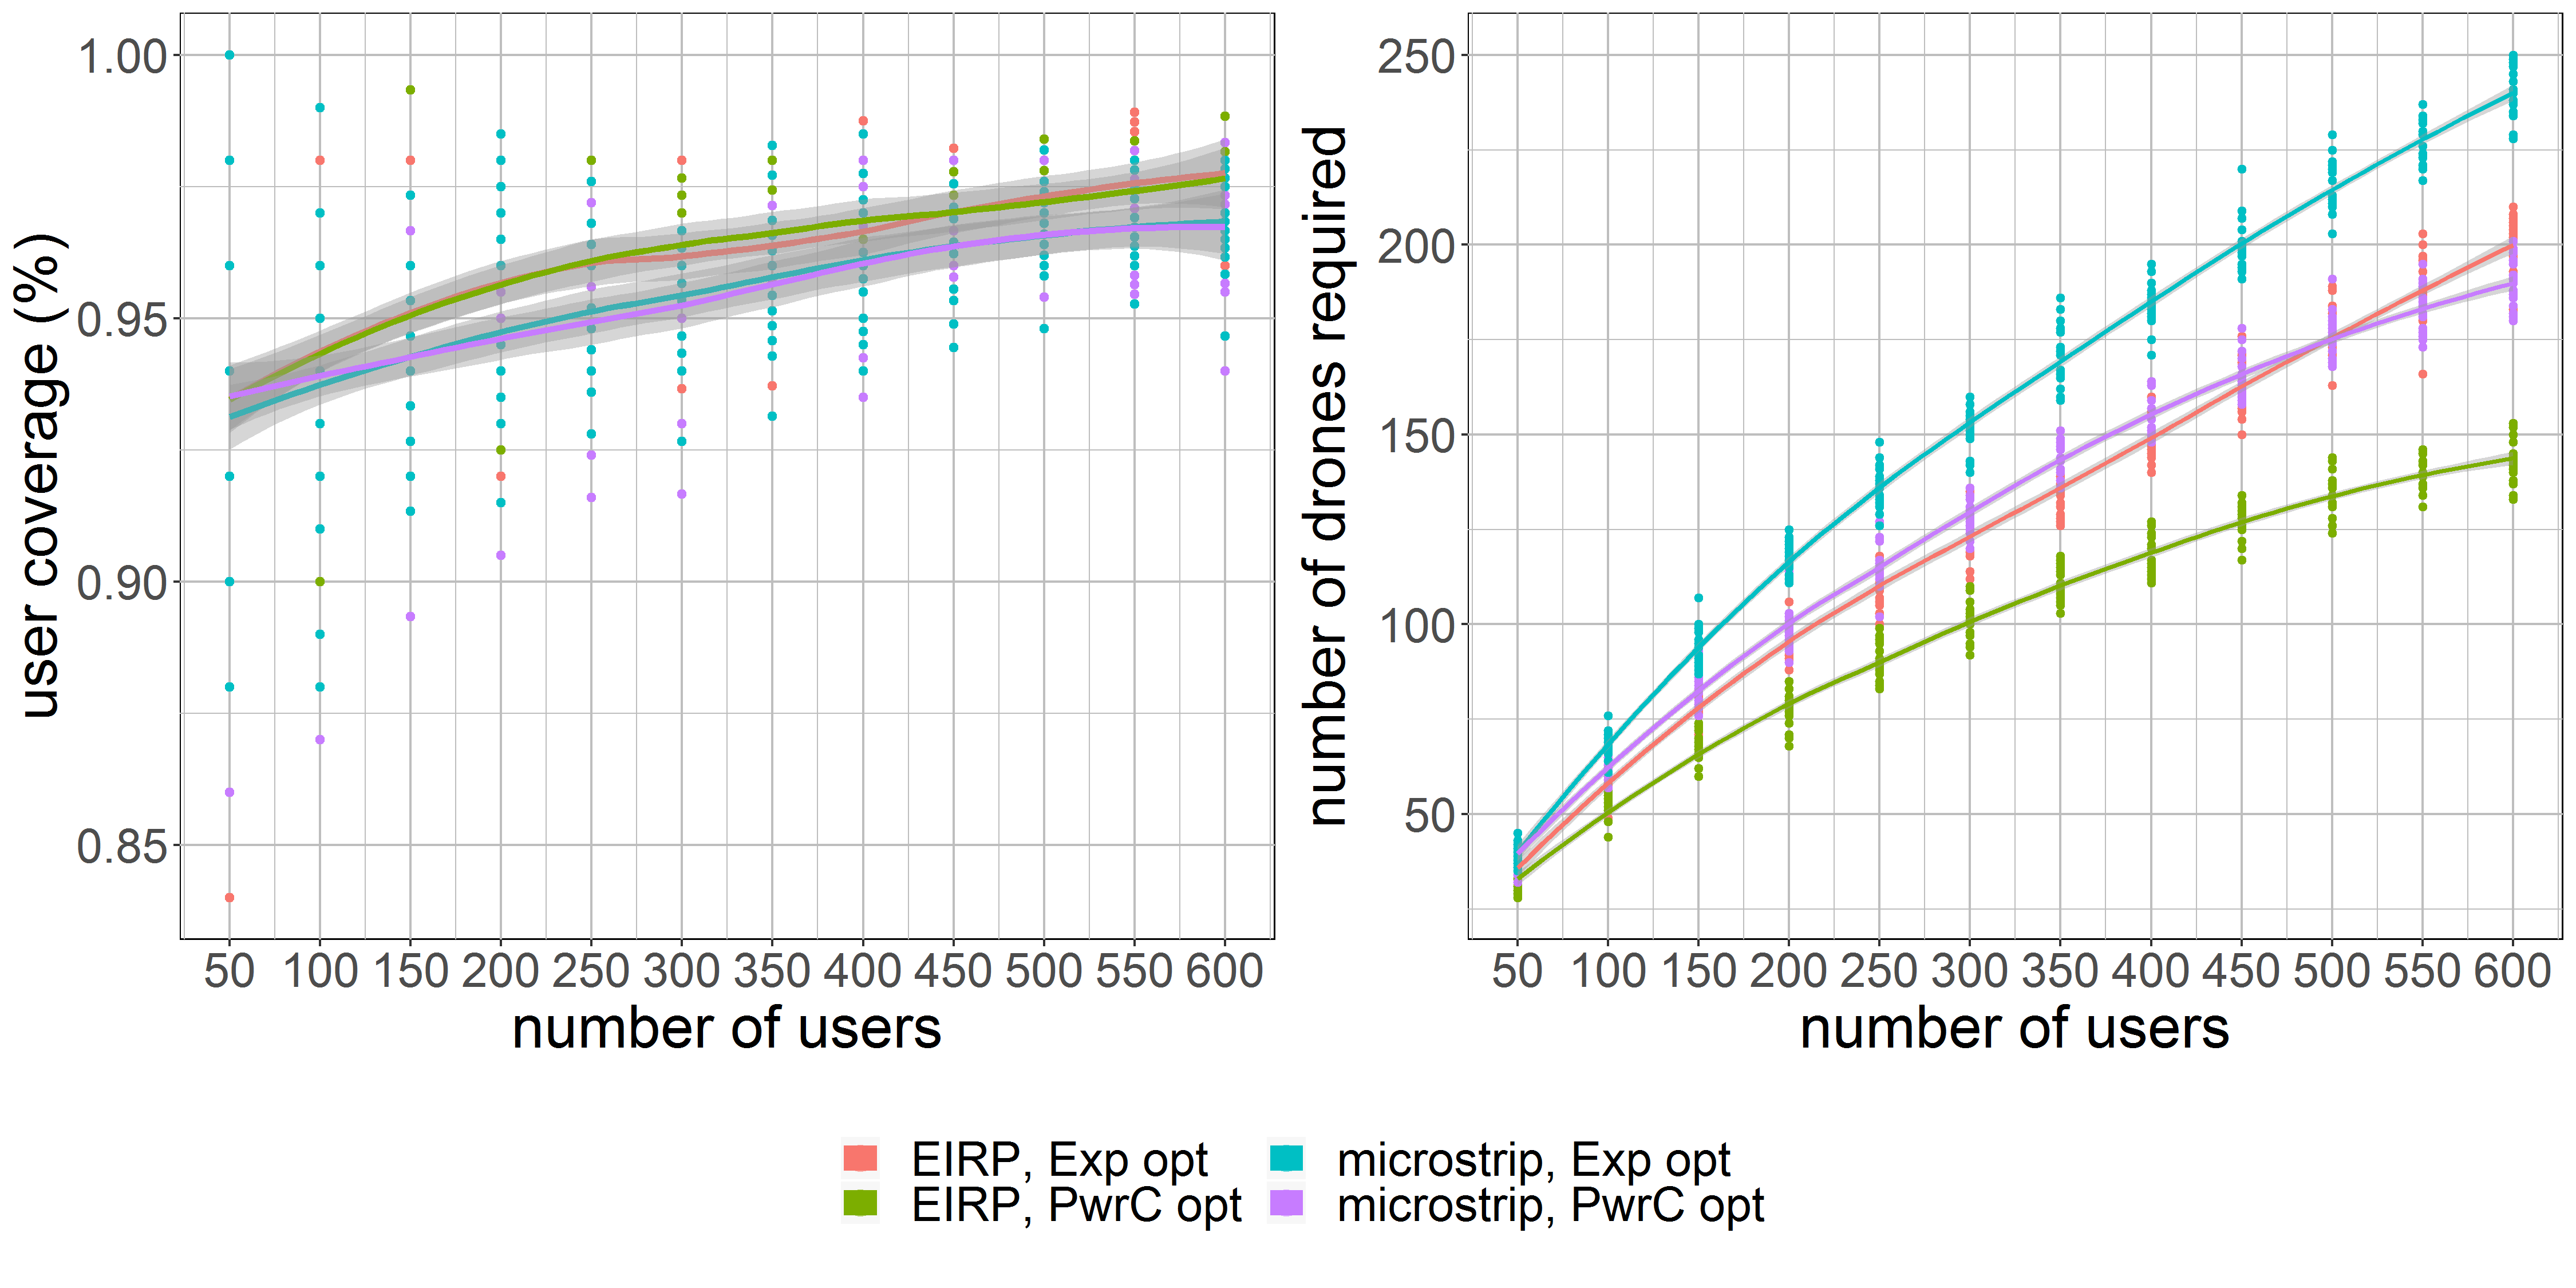
\includegraphics[width=\textwidth]{../results/s3/uvsnumdronesAndCov.png}
  \caption{This graph shows how much drones are required for different flying heights while trying to achieve a 100\% coverage.}
  \label{fig:s3b_numDronesAndCov}
\end{figure}

In a scenario with 600 active users, a clear difference is noticeable between the four configurations. 
For instance, an EIRP power consumption optimized 
network requires the least amount of drones (Figure \ref{fig:s3b_numDronesAndCov} on the right). This is logical when looking at figure \ref{fig:s3b_dlAndPC} where drones in such a configuration cause the highest amount of 
electromagnetic radiation. This behaviour was also discussed in subsection \ref{s2b}. 

So scenario 3 learns that a power consumption optimized network indeed result in very few drones. The average power consumption 
is however much higher. Scenario 2 already showed that the \gls{UABS}s who were active, have a much higher power consumption.
The statement that a power consumption optimized network will result in a few high powered devices is therefore confirmed.

Likewise for an exposure optimized network. We can that the network has indeed a lower electromagnetic exposure but the power consumption 
of the entire network is higher. In scenario 2 became already clear that the active \gls{UABS} have a low power consumption in order to 
guarantee low \gls{SAR} values for the users.  The statement that an exposure optimized network will result in a lot low powered devices is thus also confirmed.

Subsection \ref{s2b} also showed how and why a microstrip patch antennae in a low powered antenna with very little coverage. This 
explains the behaviour of our blue line. This strategy prioritize the minimization of electromagnetic exposure. Therefore much more 
drones are required in order to still reach 100\% coverage (Figure \ref{fig:s3b_numDronesAndCov}) and therefore requires much more energy 
to power all the drones (Figure \ref{fig:s3b_numDronesAndCov} on the right).
It becomes clear that more drones come with more users  and therefore result in more power consumption and electromagnetic exposure.


\begin{figure}[h!]
  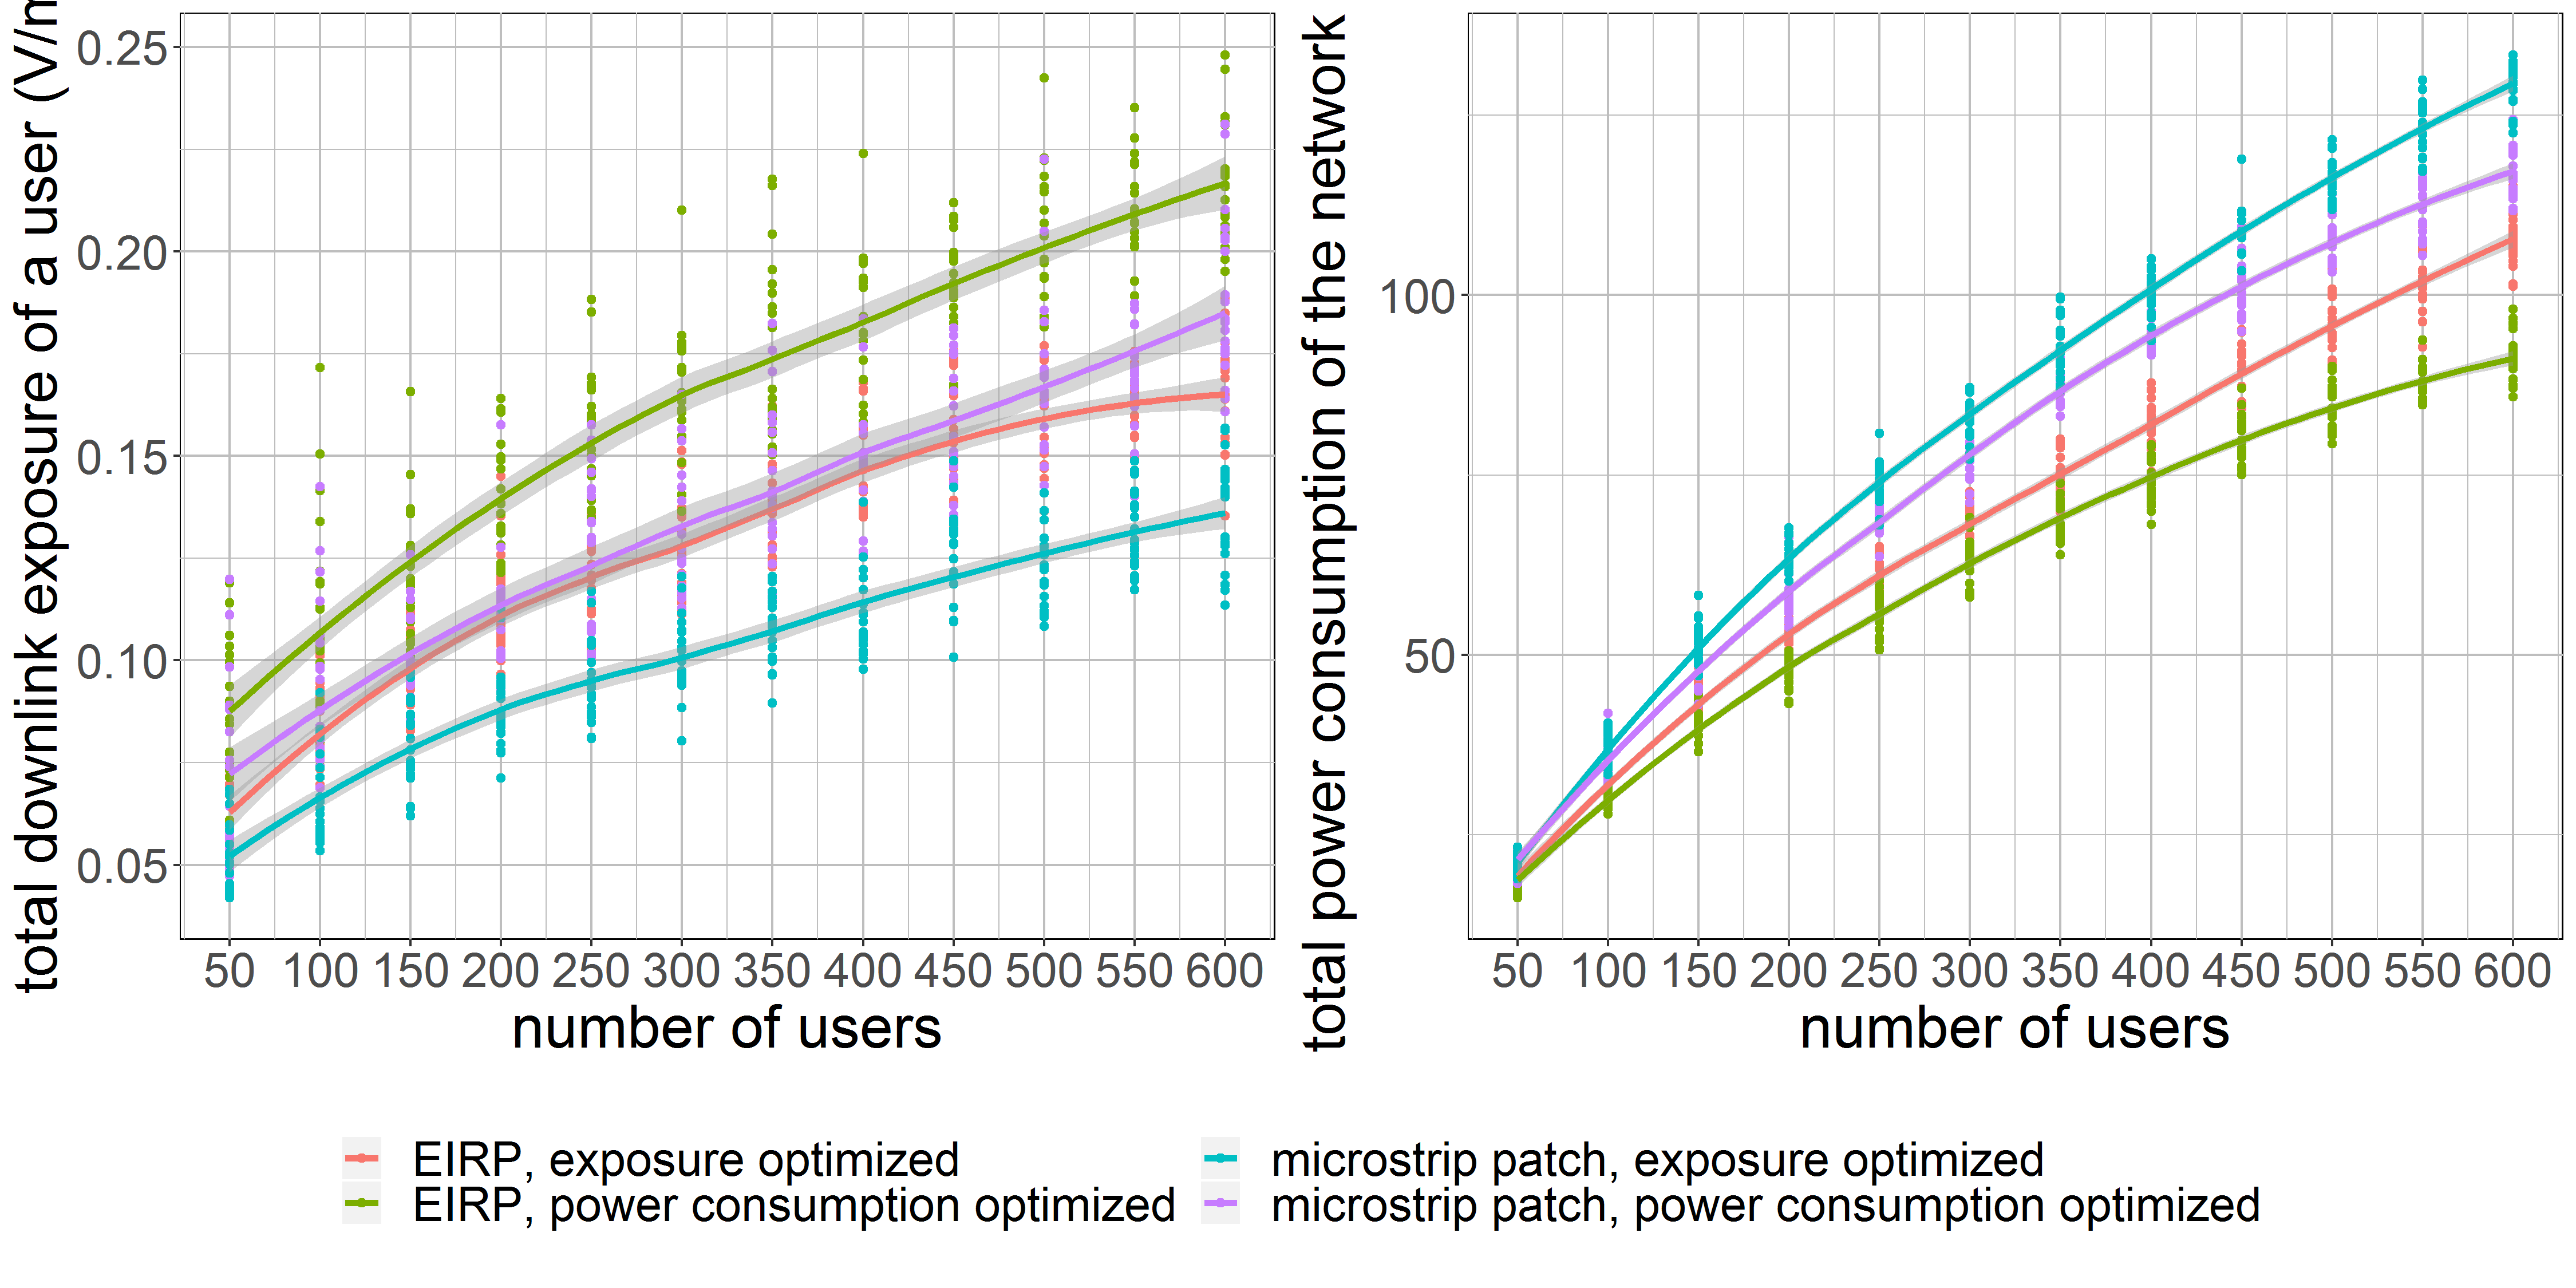
\includegraphics[width=\textwidth]{../results/s3/uvsdlAndPc.png}
  \caption{The influence of the flying height on the downlink electromagnetic radiation of the average user.}
  \label{fig:s3b_dlAndPC}
\end{figure}
todo: pc and exp inverse linear stelling van margot bevestigen

Figure \ref{fig:s3b_fourSourcesMatrix} once again shows how the \gls{SAR} from other \gls{UE} can be neglected. It increases just like before but is very 
low compared to the two other sources. Since more users result in more drones, the $SAR^{dl}_{10g}$ increases when the population 
increases. Because all drones have the same flying height, all four scenarios show at first an almost constant $SAR^{ul}_{10g}$ because the average 
distance between the user and the \gls{UABS} remain the same. However, for higher amount of users, a slightly decrease can be noticed.
Users that don't have a \gls{UABS} assigned above them still need to radiate higher to reach another \gls{UABS} nearby. The average distance 
decreases when more \gls{UABS}s are present.

\begin{figure}[h!]
  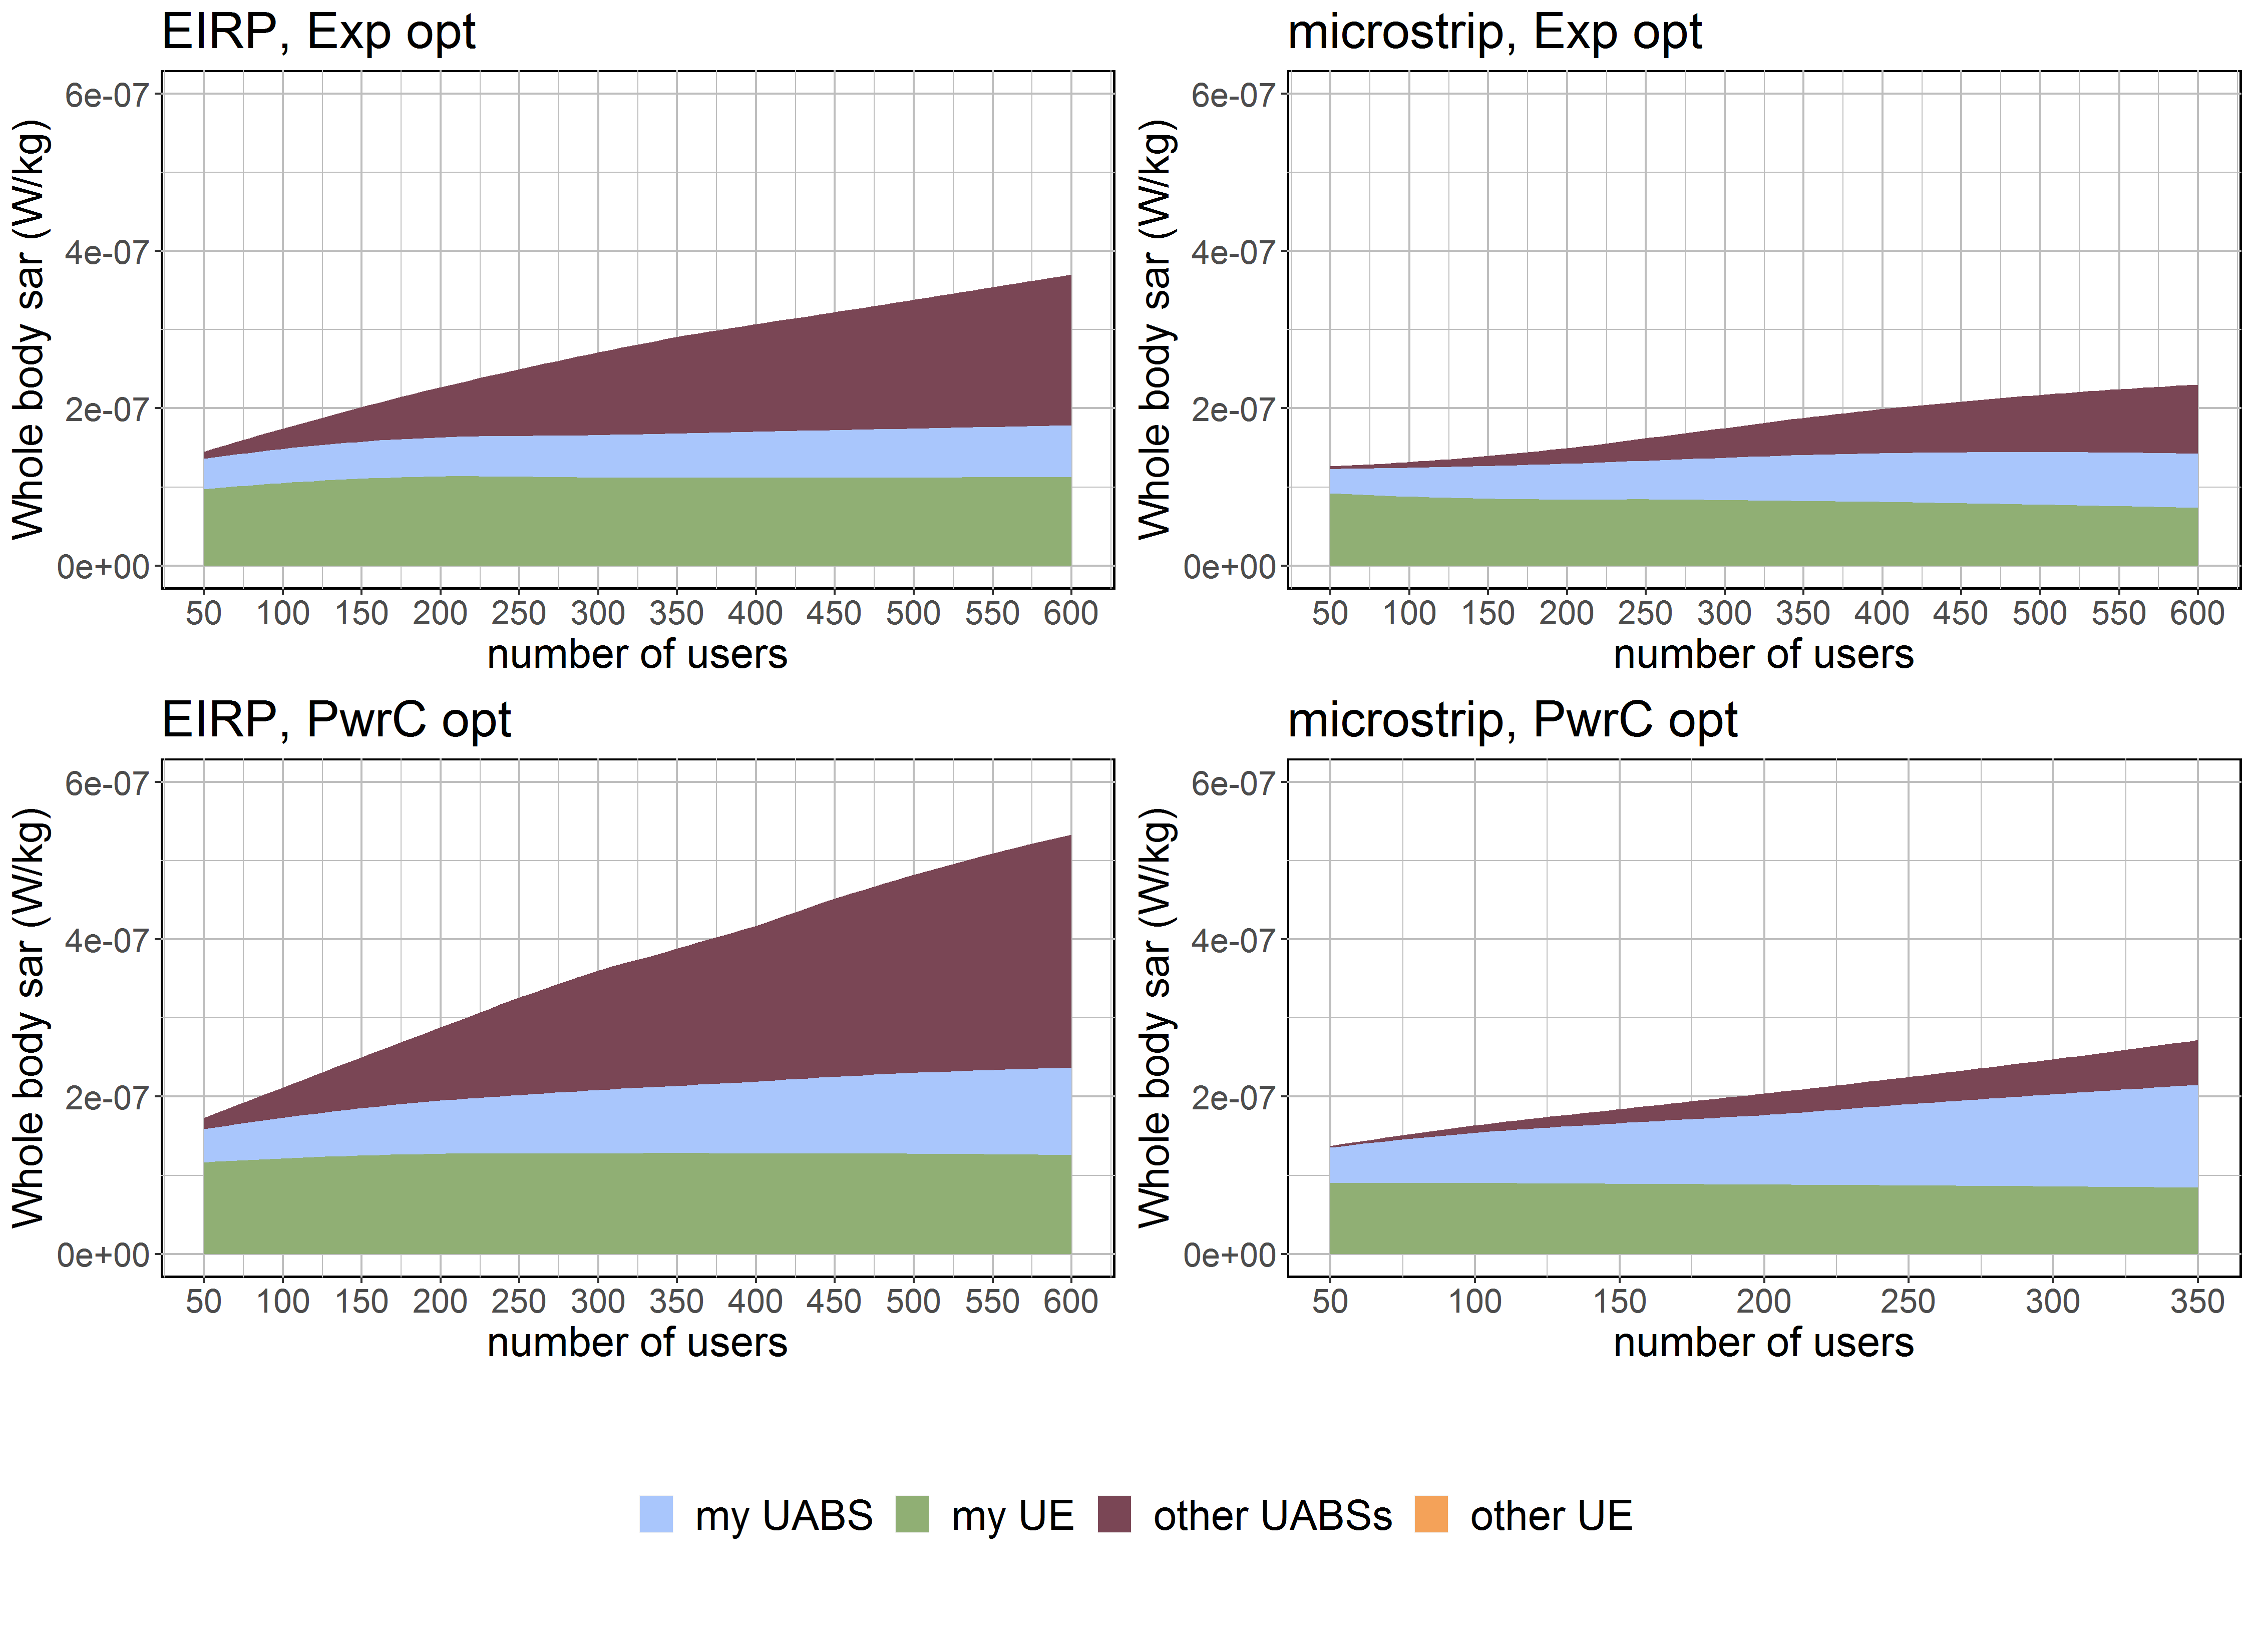
\includegraphics[width=\textwidth]{../results/s3/uFourSources.png}
  \caption{The influence of the flying height on the total power consumption of the network.}
  \label{fig:s3b_fourSourcesMatrix}
\end{figure}